%%%%%%%%%%%%%%%%%% USAGE INSTRUCTIONS %%%%%%%%%%%%%%%%%%
% - Compile using LuaLaTeX and biber, unless there is a particular reason not to. Do not use the older LaTex/PDFLaTeX or BibTeX. (The fonts won't work correctly.)
% - Expect to get 2 warnings when working correctly, one on xcolor and hyperref, and one on ExtSizes saying is better to use a class. These can be ignored.
% - Font and the report 'year' must be specified when all \documentclass or the template won't work correctly. (There's no error checking/default cases!)
% - For best performance save images/graphics as PDF files, not as png/jpg/eps. This makes no difference to how images are inserted using \includegraphics.
% - As many further packages as wanted can be loaded. Below are just an example set. Note that template itself loads a number of packages, including hyperref.
% - References are handed using biblatex.
% - Link to the presentation of dissertations policy: https://documents.manchester.ac.uk/display.aspx?DocID=2863



%%%%%%%%%%%%%%%%%% META DATA SETUP %%%%%%%%%%%%%%%%%%
% This is where the document title and author are set. Other details for the title page are set later
% Note that if/when you edit these you may need to 'Recompile from scratch' to get the changes to display in the PDF. (In Overleaf, select the down arrow to the right of the 'Recompile' button)
% [overwrite] is required: without it LaTeX silently keeps any pre-existing
% \jobname.xmpdata, so the title page and the PDF/A metadata would be taken from
% a stale file rather than from the values set here.
\begin{filecontents*}[overwrite]{\jobname.xmpdata}
  \Title{Certifying Deep Learning Classifier Predictions with High Confidence} 
  \Author{14215174} % should be student number rather than name to help with annoymous marking
  \Language{en-GB}
  \Copyrighted{True}
  % More meta-data fielda can be added here if wanted, see https://ctan.org/pkg/pdfx?lang=en for fields
\end{filecontents*}


%%%%%%%%%%%%%%%%%% DOCUMENT SETUP %%%%%%%%%%%%%%%%%%
\documentclass[11pt,msc]{uom_eee_dissertation_casson} % course can be msc or beng (MSc AI -> msc)
% Check your course handbook for the correct font size to use. Make sure this is correct - you may get an overlength penalty if not! Is currently 12 for BEng, and 11 for MSc. The template doesn't change this automatically for you


%%%%%%%%%%%%%%%%%% PACKAGES AND COMMANDS %%%%%%%%%%%%%%%%%%

% Packages
\usepackage{graphicx}              % for adding graphics files
  \graphicspath{ {./images/} }
\usepackage{amsmath}               % assumes amsmath package installed
  \allowdisplaybreaks[1]           % allow eqnarrays to break across pages
\usepackage{amssymb}               % assumes amsmath package installed 
\usepackage{url}                   % format hyperlinks correctly
\usepackage{rotating}              % allow portrait figures and tables
\usepackage{multirow}              % allows merging of rows in tables
\usepackage{lscape}                % allows pages to be typeset in landscape mode
\usepackage{tabularx}              % allows fixed width tables
\usepackage{verbatim}              % enhanced version of built-in verbatim environment
\usepackage{footnote}              % allows more control over footnote environments
\usepackage{float}                 % allows H option on floats to force here placement
\usepackage{booktabs}
\usepackage{longtable}              % improve table line spacing
\usepackage{lipsum}                % for adding dummy text here
\usepackage[base]{babel}           % required for lisum package
\usepackage{subcaption}            % for multiple sub-figures in a single float
\usepackage{siunitx}               % add SI units
% Add your packages here


% Allow TeX to stretch spacing to avoid overfull lines in text and references
\emergencystretch=3em
\hbadness=10000  % silence underfull-hbox info from the stretching

% The class loads hyperref before amsmath, so the stored equation label is
% already parenthesised ("(2)"); amsmath's \eqref would add a second pair and
% print "((2))". Referring through \ref gives the single, correct "(2)".
\renewcommand{\eqref}[1]{\textup{\ref{#1}}}

% Custom commands
\newcommand{\degree}{\ensuremath{^\circ}}
\newcommand{\sus}[1]{$^{\mbox{\scriptsize #1}}$} % superscript in text (e.g. 1st)
\newcommand{\sub}[1]{$_{\mbox{\scriptsize #1}}$} % subscript in text
\newcommand{\otoprule}{\midrule[\heavyrulewidth]}
\newcolumntype{Z}{>{\centering\arraybackslash}X}  % tabularx centered columns 
% Add your custom commands here



%%%%%%%%%%%%%%%%%% REFERENCES SETUP %%%%%%%%%%%%%%%%%%

% Setup your references here. Change the reference style here if wanted
\usepackage[style=numeric,backend=biber,backref=true,hyperref=auto,maxbibnames=3,minbibnames=1]{biblatex}
% Note backref=true adds a page number (and hyperlink) to each reference so you can easily go back from the references to the main document. You may prefer backref=false if you need to stick strictly to a given reference style


% Fixes which can't be applied in the .cls file
\DefineBibliographyStrings{english}{backrefpage = {cited on p\adddot},  backrefpages = {cited on pp\adddot}}
%  \renewcommand*{\bibfont}{\large}


% Add more .bib files here if wanted
\addbibresource{references.bib}

% Registry-generated inline numbers (mean values); regenerated by scripts/gen_tables.py
\IfFileExists{generated/numbers.tex}{% AUTO-GENERATED from results/processed/summary.csv -- do not edit.
% Usage: \certMnistFcnFquadLearnt etc. (mean, 4 dp).
\providecommand{\nresult}[1]{#1}
\newcommand{\CertCifaronezeroCnnBbbLearnt}{0.9801}
\newcommand{\StochCifaronezeroCnnBbbLearnt}{0.2412}
\newcommand{\PostmeanCifaronezeroCnnBbbLearnt}{0.2162}
\newcommand{\KlCifaronezeroCnnBbbLearnt}{83760.2141}
\newcommand{\NboundCifaronezeroCnnBbbLearnt}{25000}
\newcommand{\EmpCifaronezeroCnnBbbLearnt}{0.0767}
\newcommand{\CertCifaronezeroCnnFclassicLearnt}{0.3932}
\newcommand{\StochCifaronezeroCnnFclassicLearnt}{0.2902}
\newcommand{\PostmeanCifaronezeroCnnFclassicLearnt}{0.2615}
\newcommand{\KlCifaronezeroCnnFclassicLearnt}{292.2373}
\newcommand{\NboundCifaronezeroCnnFclassicLearnt}{25000}
\newcommand{\EmpCifaronezeroCnnFclassicLearnt}{0.3174}
\newcommand{\CertCifaronezeroCnnFquadLearnt}{0.4277}
\newcommand{\StochCifaronezeroCnnFquadLearnt}{0.2802}
\newcommand{\PostmeanCifaronezeroCnnFquadLearnt}{0.2525}
\newcommand{\KlCifaronezeroCnnFquadLearnt}{843.2009}
\newcommand{\NboundCifaronezeroCnnFquadLearnt}{25000}
\newcommand{\EmpCifaronezeroCnnFquadLearnt}{0.3003}
\newcommand{\CertCifaronezeroCnnFquadRand}{0.9297}
\newcommand{\StochCifaronezeroCnnFquadRand}{0.8978}
\newcommand{\PostmeanCifaronezeroCnnFquadRand}{0.9000}
\newcommand{\KlCifaronezeroCnnFquadRand}{14.3337}
\newcommand{\NboundCifaronezeroCnnFquadRand}{50000}
\newcommand{\EmpCifaronezeroCnnFquadRand}{0.9203}
\newcommand{\CertCifaronezeroCnnonethreeFquadLearnt}{0.3881}
\newcommand{\StochCifaronezeroCnnonethreeFquadLearnt}{0.2202}
\newcommand{\PostmeanCifaronezeroCnnonethreeFquadLearnt}{0.1791}
\newcommand{\KlCifaronezeroCnnonethreeFquadLearnt}{1189.9267}
\newcommand{\NboundCifaronezeroCnnonethreeFquadLearnt}{25000}
\newcommand{\EmpCifaronezeroCnnonethreeFquadLearnt}{0.2416}
\newcommand{\CertCifaronezeroCnnonefiveFquadLearnt}{0.4722}
\newcommand{\StochCifaronezeroCnnonefiveFquadLearnt}{0.2847}
\newcommand{\PostmeanCifaronezeroCnnonefiveFquadLearnt}{0.2265}
\newcommand{\KlCifaronezeroCnnonefiveFquadLearnt}{1296.9336}
\newcommand{\NboundCifaronezeroCnnonefiveFquadLearnt}{25000}
\newcommand{\EmpCifaronezeroCnnonefiveFquadLearnt}{0.3134}
\newcommand{\CertFashionmnistCnnFquadLearnt}{0.1674}
\newcommand{\StochFashionmnistCnnFquadLearnt}{0.0931}
\newcommand{\PostmeanFashionmnistCnnFquadLearnt}{0.0866}
\newcommand{\KlFashionmnistCnnFquadLearnt}{423.3348}
\newcommand{\NboundFashionmnistCnnFquadLearnt}{30000}
\newcommand{\EmpFashionmnistCnnFquadLearnt}{0.1069}
\newcommand{\CertFashionmnistFcnBbbLearnt}{0.6632}
\newcommand{\StochFashionmnistFcnBbbLearnt}{0.1118}
\newcommand{\PostmeanFashionmnistFcnBbbLearnt}{0.1018}
\newcommand{\KlFashionmnistFcnBbbLearnt}{21606.3770}
\newcommand{\NboundFashionmnistFcnBbbLearnt}{30000}
\newcommand{\EmpFashionmnistFcnBbbLearnt}{0.0913}
\newcommand{\CertFashionmnistFcnFclassicLearnt}{0.1582}
\newcommand{\StochFashionmnistFcnFclassicLearnt}{0.1204}
\newcommand{\PostmeanFashionmnistFcnFclassicLearnt}{0.1136}
\newcommand{\KlFashionmnistFcnFclassicLearnt}{26.1967}
\newcommand{\NboundFashionmnistFcnFclassicLearnt}{30000}
\newcommand{\EmpFashionmnistFcnFclassicLearnt}{0.1387}
\newcommand{\CertFashionmnistFcnFquadLearnt}{0.1746}
\newcommand{\StochFashionmnistFcnFquadLearnt}{0.1186}
\newcommand{\PostmeanFashionmnistFcnFquadLearnt}{0.1109}
\newcommand{\KlFashionmnistFcnFquadLearnt}{157.9383}
\newcommand{\NboundFashionmnistFcnFquadLearnt}{30000}
\newcommand{\EmpFashionmnistFcnFquadLearnt}{0.1349}
\newcommand{\CertFashionmnistFcnFquadRand}{0.4480}
\newcommand{\StochFashionmnistFcnFquadRand}{0.2254}
\newcommand{\PostmeanFashionmnistFcnFquadRand}{0.1891}
\newcommand{\KlFashionmnistFcnFquadRand}{5236.9718}
\newcommand{\NboundFashionmnistFcnFquadRand}{60000}
\newcommand{\EmpFashionmnistFcnFquadRand}{0.2461}
\newcommand{\CertMnistCnnFquadLearnt}{0.0369}
\newcommand{\StochMnistCnnFquadLearnt}{0.0108}
\newcommand{\PostmeanMnistCnnFquadLearnt}{0.0095}
\newcommand{\KlMnistCnnFquadLearnt}{124.2753}
\newcommand{\NboundMnistCnnFquadLearnt}{30000}
\newcommand{\EmpMnistCnnFquadLearnt}{0.0201}
\newcommand{\CertMnistFcnBbbLearnt}{0.2658}
\newcommand{\StochMnistFcnBbbLearnt}{0.0187}
\newcommand{\PostmeanMnistFcnBbbLearnt}{0.0149}
\newcommand{\KlMnistFcnBbbLearnt}{7483.5041}
\newcommand{\NboundMnistFcnBbbLearnt}{30000}
\newcommand{\EmpMnistFcnBbbLearnt}{0.0138}
\newcommand{\CertMnistFcnFclassicLearnt}{0.0455}
\newcommand{\StochMnistFcnFclassicLearnt}{0.0240}
\newcommand{\PostmeanMnistFcnFclassicLearnt}{0.0192}
\newcommand{\KlMnistFcnFclassicLearnt}{6.6281}
\newcommand{\NboundMnistFcnFclassicLearnt}{30000}
\newcommand{\EmpMnistFcnFclassicLearnt}{0.0373}
\newcommand{\CertMnistFcnFlambLearnt}{0.0777}
\newcommand{\StochMnistFcnFlambLearnt}{0.0211}
\newcommand{\PostmeanMnistFcnFlambLearnt}{0.0170}
\newcommand{\KlMnistFcnFlambLearnt}{609.6926}
\newcommand{\NboundMnistFcnFlambLearnt}{30000}
\newcommand{\EmpMnistFcnFlambLearnt}{0.0294}
\newcommand{\CertMnistFcnFquadLearntPtOneZero}{0.1520}
\newcommand{\StochMnistFcnFquadLearntPtOneZero}{0.0632}
\newcommand{\PostmeanMnistFcnFquadLearntPtOneZero}{0.0551}
\newcommand{\KlMnistFcnFquadLearntPtOneZero}{60.3676}
\newcommand{\NboundMnistFcnFquadLearntPtOneZero}{3000}
\newcommand{\EmpMnistFcnFquadLearntPtOneZero}{0.0771}
\newcommand{\CertMnistFcnFquadLearntPtTwoZero}{0.1196}
\newcommand{\StochMnistFcnFquadLearntPtTwoZero}{0.0468}
\newcommand{\PostmeanMnistFcnFquadLearntPtTwoZero}{0.0388}
\newcommand{\KlMnistFcnFquadLearntPtTwoZero}{93.4216}
\newcommand{\NboundMnistFcnFquadLearntPtTwoZero}{6000}
\newcommand{\EmpMnistFcnFquadLearntPtTwoZero}{0.0624}
\newcommand{\CertMnistFcnFquadLearntPtFiveZero}{0.0777}
\newcommand{\StochMnistFcnFquadLearntPtFiveZero}{0.0304}
\newcommand{\PostmeanMnistFcnFquadLearntPtFiveZero}{0.0236}
\newcommand{\KlMnistFcnFquadLearntPtFiveZero}{141.0838}
\newcommand{\NboundMnistFcnFquadLearntPtFiveZero}{15000}
\newcommand{\EmpMnistFcnFquadLearntPtFiveZero}{0.0420}
\newcommand{\CertMnistFcnFquadLearnt}{0.0580}
\newcommand{\StochMnistFcnFquadLearnt}{0.0219}
\newcommand{\PostmeanMnistFcnFquadLearnt}{0.0176}
\newcommand{\KlMnistFcnFquadLearnt}{187.4999}
\newcommand{\NboundMnistFcnFquadLearnt}{30000}
\newcommand{\EmpMnistFcnFquadLearnt}{0.0328}
\newcommand{\CertMnistFcnFquadLearntLnOneZero}{0.2334}
\newcommand{\StochMnistFcnFquadLearntLnOneZero}{0.0608}
\newcommand{\PostmeanMnistFcnFquadLearntLnOneZero}{0.0553}
\newcommand{\KlMnistFcnFquadLearntLnOneZero}{219.6397}
\newcommand{\NboundMnistFcnFquadLearntLnOneZero}{30000}
\newcommand{\EmpMnistFcnFquadLearntLnOneZero}{0.1816}
\newcommand{\CertMnistFcnFquadLearntLnTwoZero}{0.4289}
\newcommand{\StochMnistFcnFquadLearntLnTwoZero}{0.1165}
\newcommand{\PostmeanMnistFcnFquadLearntLnTwoZero}{0.1112}
\newcommand{\KlMnistFcnFquadLearntLnTwoZero}{676.3138}
\newcommand{\NboundMnistFcnFquadLearntLnTwoZero}{30000}
\newcommand{\EmpMnistFcnFquadLearntLnTwoZero}{0.3240}
\newcommand{\CertMnistFcnFquadLearntLnFourZero}{0.7013}
\newcommand{\StochMnistFcnFquadLearntLnFourZero}{0.2647}
\newcommand{\PostmeanMnistFcnFquadLearntLnFourZero}{0.2550}
\newcommand{\KlMnistFcnFquadLearntLnFourZero}{974.5434}
\newcommand{\NboundMnistFcnFquadLearntLnFourZero}{30000}
\newcommand{\EmpMnistFcnFquadLearntLnFourZero}{0.5799}
\newcommand{\CertMnistFcnFquadRand}{0.3496}
\newcommand{\StochMnistFcnFquadRand}{0.0927}
\newcommand{\PostmeanMnistFcnFquadRand}{0.0570}
\newcommand{\KlMnistFcnFquadRand}{8258.0648}
\newcommand{\NboundMnistFcnFquadRand}{60000}
\newcommand{\EmpMnistFcnFquadRand}{0.1199}
\newcommand{\ReproStochDeltaMin}{-0.0024}
\newcommand{\ReproStochDeltaMax}{+0.0033}
\newcommand{\ReproStochDeltaAbsMax}{0.0033}
\newcommand{\ReproCertDeltaMin}{+0.0214}
\newcommand{\ReproCertDeltaMax}{+0.0423}
\newcommand{\ReproCertDeltaAbsMax}{0.0423}
}{}



%%%%%%%%%%%%%%%%%% AUTOMATIC WORD COUNT SETUP %%%%%%%%%%%%%%%%%%
% Automatically counts the words present and makes a \mywordcount variable. This is used later to automatically add the word count (which can be overridden if wanted)
% See https://www.overleaf.com/learn/how-to/Is_there_a_way_to_run_a_word_count_that_doesn%27t_include_LaTeX_commands%3F for info on what words are counted and how to control this. Any changes to what's counted need to be made in uom_thesis_casson.cls, in the \newcommand{\quickwordcount} command. The default doesn't count words in headings, captions, or references and so you may get slightly different numbers if use a different word count tool
% This can be a bit fragile. If it doesn't work, there's an option later on to just type in a numer
%\quickwordcount disabled (texcount unavailable) % run word count. This just counts the words. Is displayed with the \wordcount command later



%%%%%%%%%%%%%%%%%% START DOCUMENT %%%%%%%%%%%%%%%%%%

% Don't edit these lines, title and author are automatically taken from the document meta-data defined above
\begin{document}
\makeatletter
\title{\xmp@Title}
\studentid{\xmp@Author}
\makeatother

% Set the below yourself
\course{Artificial Intelligence}  % "Master of Science in" or "Bachelor of Engineering in "
                                                   % is added automatically
                                                   % Our BEng courses are: Electrical and Electronic Engineering, Electrical Engineering, and Mechatronic Engineering
                                                   % Our MSc courses are: Advanced Control and Systems Engineering, Advanced Control and Systems Engineering with Extended Research, Communications and Signal Processing, Communications and Signal Processing with Extended Research, Electrical Power Systems Engineering, Advanced Electrical Power Systems Engineering, Renewable Energy and Clean Technology, Renewable Energy and Clean Technology with Extended Research, Robotics, Robotics with Extended Research
\faculty{Science and Engineering}                  % "Faculty of" is added automatically
\school{School of Engineering} % "School of" not added automatically (as if in AMBS, School comes at the end rather than the start), so enter full name of School here
\submitdate{2026}                                  % regulations ask only for the year, not month
\wordcount{8948}                                   % abstract + Sections 1-6, measured with
                                                   % texcount; excludes references, appendices
                                                   % and figure/table captions per the rubric
\maketitle



%%%%%%%%%%%%%%%%%% LISTS OF CONTENT %%%%%%%%%%%%%%%%%%
\uomtoc
% other lists are not required, but can include \uomlof and \uomlot if really want to


%%%%%%%%%%%%%%%%%% ABSTRACT %%%%%%%%%%%%%%%%%%
\begin{abstract}
A classifier's test-set error gives no high-confidence guarantee about its true
risk. PAC-Bayes theory provides such guarantees, called risk certificates, for
stochastic predictors, and the PAC-Bayes-with-Backprop (PBB) framework of
\textcite{perezortiz2021} makes them numerically non-vacuous for deep networks by
training the weight distribution to minimise the bound directly. A certificate is
only valid, however, if every step of its computation is correct. This
dissertation re-implements that computation from scratch, reproduces four MNIST
cells of the reference under a reduced-compute protocol, and extends the same
pipeline to Fashion-MNIST and CIFAR-10.

We found and corrected five issues in the reference implementation, each under a
unit test: three change the reported certificate (the bound-set sample count, the
batched Monte-Carlo aggregation and the joint confidence accounting), one affects
reproducibility (seed control), and one decides whether the learnt prior is
admissible at all, since a class-stratified partition makes the prior depend on
the very labels the bound is evaluated on. We additionally correct for a
selection of our own: the prior scale was settled by comparing certificates on
the bound set, so every certificate carries a union over a grid of candidate
prior scales, under a stated assumption we carry as a threat rather than a
settled matter.

Over five seeds the reproduction matches the published stochastic test errors to
within $\ReproStochDeltaAbsMax$ on all four target cells, while our certificates
are looser by $\ReproCertDeltaMin$ to $\ReproCertDeltaMax$; re-drawing at the
reference's full Monte-Carlo budget recovers a little over half of that gap on
the checkpoint examined, and the remainder is left unattributed. The learnt-prior
MNIST certificates are non-vacuous ($f_{\text{classic}}$
$\CertMnistFcnFclassicLearnt$, $f_{\text{quad}}$ $\CertMnistFcnFquadLearnt$) and
loosen to $\CertFashionmnistFcnFquadLearnt$ on Fashion-MNIST and
$\CertCifaronezeroCnnFquadLearnt$ on CIFAR-10, where the 13-layer network is
tightest ($\CertCifaronezeroCnnonethreeFquadLearnt$) and the 15-layer one trains
only three seeds in five. A data-dependent prior tightens the certificate in all
three paired controls, though not by the same mechanism in each, and the
accuracy-oriented Bayes-by-Backprop baseline attains the best test error and the
loosest certificate: tightness tracks not accuracy but how much KL an objective
spends to reach it. Decomposing the certified risk by class shows it is far from
evenly spread, one Fashion-MNIST class carrying $0.293$ against a dataset-wide
$0.108$. We certify only the Gibbs classifier, and release an artefact in which
every reported number is regenerated from a results registry. The main
contribution is the corrected, tested pipeline, since the value of any
certificate depends on the sample counts, confidence accounting and Monte-Carlo
aggregation that produce it.

\end{abstract}%
\clearpage



%%%%%%%%%%%%%%%%%% DECLARATIONS %%%%%%%%%%%%%%%%%%
\begin{uomoriginality}
  \uomoriginalitydeclaration 
  % If the standard originality decalaration is sufficient, saying no portion of the work has been submitted in support of an application for another degree or qualification, the above command will automatically add the required text and nothing else is needed in this section.
  % If the standard statment isn't sufficient, then comment out the \uomoriginalitydeclaration command and type in your own text here explaining the authorship of any re-used portions. 
\end{uomoriginality}
\uomcopyrightstatement



%%%%%%%%%%%%%%%%%% ACKNOWLEDGEMENTS %%%%%%%%%%%%%%%%%%
\begin{uomacknowledgements}
I thank my supervisor, Dr.\ Omar Rivasplata, for detailed feedback on the
correctness of the risk certificates and on the reproducibility of the
experimental pipeline. This work
builds on the open-source PAC-Bayes-with-Backprop implementation of
P\'erez-Ortiz et al.\ (2021); the public MNIST, Fashion-MNIST and CIFAR-10
benchmarks were used throughout. Generative AI tools were used in the course
of the project: OpenAI Codex to review the experiment code before the
experiments were run, and GPT-5.6, through the ChatGPT interface, to review
this report and to edit its language. Their use is declared in full in the
accompanying declaration of generative AI use.
\end{uomacknowledgements}



%%%%%%%%%%%%%%%%%% Start content %%%%%%%%%%%%%%%%%%
\uomstartmainbody

% Full rewrite (supervisor feedback): RQ-driven, Gibbs-only certificate scope,
% honest joint confidence, corrected sample accounting, registry-generated numbers.
\section{Introduction}\label{sec:intro}

\subsection{Motivation}\label{sec:motivation}

When a neural network is reported to reach, say, $98\%$ accuracy on a benchmark,
that figure is an estimate from one finite test set. It carries no stated
confidence, it varies from one test split to another, and it can be quietly
inflated when the same test set is consulted repeatedly during model selection.
For a deployed classifier we often want something stronger: ``with probability
at least $99\%$, the expected error of this model is below $r$''. A bound of this
kind is a \emph{risk certificate}, computed from the training data and the
learning algorithm rather than from a held-out test set.

PAC-Bayes theory \parencite{mcallester1999,seeger2002,catoni2007} is the main
route to such guarantees, for \emph{stochastic} predictors whose weights are
drawn from a distribution $Q$ learnt from data.
For a long time these bounds were of theoretical interest only: applied to a
modern over-parameterised network they returned values above one, which certify
nothing. That changed when the bound was used not merely to analyse a
trained model but to \emph{train} it. PAC-Bayes-with-Backprop (PBB)
\parencite{perezortiz2021} optimises the weight distribution by minimising a
PAC-Bayes bound directly, obtaining certificates that are numerically meaningful
and competitive in accuracy. This project reproduces that framework,
extends it to two further datasets, and examines how trustworthy the resulting
certificates are once the computation behind them is scrutinised.

\subsection{Why certificate reproduction is hard}\label{sec:problem}

A test-error number is forgiving: a small mistake in computing it usually produces
a slightly wrong but still plausible figure. A certificate is not. Its validity
rests on a chain of conditions that must all hold at once. The empirical risk
inside the bound has to be measured on data the prior never saw, and the sample
size dividing the complexity term has to be the size of that held-out set rather
than of the whole dataset. The risk of a stochastic predictor has no closed form,
so it is estimated by Monte-Carlo sampling, which introduces a second failure
probability that must be combined with the PAC-Bayes one. And the object certified
is the stochastic (Gibbs) classifier, not the deterministic network a practitioner
deploys. Handle any of these wrongly and the pipeline still produces a number that
looks like a certificate, but it no longer holds.

We therefore re-implement the pipeline from first principles alongside
reproducing and extending PBB, and test each condition explicitly. That surfaced
several points at which the reference implementation departs from them; we
correct those and recompute every certificate accordingly.

\subsection{Subject area and key related work}\label{sec:related}

Non-vacuous numerical bounds go back to \textcite{langford2001}, for small
networks only. The modern line begins with \textcite{dziugaite2017}: a
deterministic network has a point-mass weight distribution, for which the
PAC-Bayes complexity term is infinite, so by spreading the weights into a Gaussian
and optimising the spread they turned an infinite penalty into a finite one and
reported the first non-vacuous bound (around $0.21$) on MNIST. It was loose, but
it established that the approach was numerically viable.

Two factors separate a loose bound from a tight one, and both matter here. The
first is keeping the posterior $Q$ close to the prior $P$, since the bound
penalises their KL divergence, and a prior fixed before seeing any data sits far
from any well-trained posterior. \textcite{dziugaite2018} addressed this by making
the prior depend on the data through differential privacy, and
\textcite{rivasplata2018} analysed instance-dependent priors more generally; both
show that moving the prior towards the data shrinks the KL substantially. The
second is to optimise the bound itself. \textcite{perezortiz2021}, the work this
project reproduces, trains $Q$ by minimising one of three surrogate PAC-Bayes
objectives (a McAllester/Pinsker form $f_{\text{classic}}$, the Catoni-style bound
of \textcite{thiemann2017} $f_{\lambda}$, and a quadratic relaxation
$f_{\text{quad}}$), combined with a prior learnt on a held-out portion of the
training data, and reports $0$--$1$ certificates around $0.02$--$0.03$ on MNIST,
an order of magnitude tighter than \textcite{dziugaite2017}, at good accuracy.
Later work develops the self-certified and learnt-prior settings
\parencite{perezortiz2021b,perezortiz2021c}, and \textcite{garciaperez2025}
tightens the underlying inequalities.

Which predictor the bound controls matters throughout what follows: it is a
statement about the Gibbs classifier, which resamples weights for each
prediction. Transferring it to the deterministic majority vote is possible in
principle through the C-bound \parencite{lacasse2006,germain2015}, which relates
the majority-vote risk to the mean and variance of the Gibbs risk, but that is a
different and generally looser statement. The baseline we compare against,
Bayes-by-Backprop \parencite{blundell2015}, learns a Gaussian posterior by
maximising a variational objective rather than a risk bound, and so achieves
strong accuracy without a tight certificate. More broadly, deep ensembles
\parencite{lakshminarayanan2017}, MC-dropout \parencite{gal2016} and post-hoc
calibration \parencite{guo2017} quantify uncertainty empirically without a
distribution-free guarantee on the risk, while randomised smoothing
\parencite{cohen2019} certifies a different, adversarial quantity.

\subsection{Objectives}\label{sec:rqs}

The project brief is to reproduce the PBB experiments on MNIST, extend them to
Fashion-MNIST, and analyse CIFAR-10. Within that brief the technical work pursues
four questions. The first is one of \emph{reproduction fidelity}: under an
explicitly reduced compute budget, how closely does a corrected, independent
re-implementation match the reference's MNIST results when the same metrics are
compared? To make that decidable rather than a matter of impression, targets and
tolerance are fixed in advance: four MNIST cells of the reference's Table~1 --- FCN
with a data-free prior under $f_{\text{quad}}$, FCN with a learnt prior under
$f_{\text{quad}}$ and under $f_{\lambda}$, and CNN with a learnt prior under
$f_{\text{quad}}$ --- each counting as reproduced when our mean stochastic test
error is within one percentage
point of the published value. We set \emph{no} tolerance on the certificate,
because one computed at $m=2{,}000$ is not the same quantity as one computed at
$m=150{,}000$; instead we report the gap per cell and measure how much of it the
Monte-Carlo budget explains. The second concerns the \emph{anatomy} of the certificate, namely how
the empirical Gibbs risk, the KL term and the bound-set size $n_{\mathrm b}$ each
contribute to the final value across the three datasets, and how a learnt prior
shifts that balance. Building on this, the third asks how \emph{sensitive} the
certificate is to the choices around it: the prior family, the amount of training
data, the Monte-Carlo budget, the random seed, and the sample-count convention
that the audit corrects. The last isolates a single notion of difficulty: with the
architecture, sample size and compute held fixed, does injected label noise move
the empirical-risk, KL and certificate terms together, so that a difficulty effect
can be separated from the confounds of a cross-dataset comparison?

The dissertation makes five contributions. It (i) reproduces the principal PBB
MNIST cells under a documented, reduced-compute protocol and compares them with the
published numbers on identically-defined metrics; (ii) extends the same pipeline to
Fashion-MNIST and CIFAR-10, adding the learnt-versus-random prior contrast on every
dataset, a CIFAR-10 random-prior control the original study did not report, and
its 13- and 15-layer CIFAR-10 architectures, at the deeper of which the fixed
configuration begins to fail to train;
(iii) identifies, in the public reference \emph{implementation} and not in the
theory of \textcite{perezortiz2021}, whose inequalities we use unchanged, five
issues in the certificate pipeline, and corrects each under a unit test: three
change the certificate value (the bound-set sample count, the batched Monte-Carlo
aggregation, the joint confidence accounting), one affects reproducibility (seed
control) and one affects whether the learnt-prior construction meets the
independence condition at all (a label-independent partition). It also pays for a
step of its own, since the prior scale was chosen by comparing certificates on
the bound set, with a union over a grid of candidate prior scales, and states
precisely what that correction does and does not settle;
(iv) decomposes certificate behaviour into its empirical-risk, KL, sample-size and
Monte-Carlo components, by class, and under a controlled label-noise perturbation;
and (v) releases a reproducible artefact in which every results figure and
reported number is generated from a results registry with per-run provenance and an
inclusion/exclusion record.

\subsection{Report structure}\label{sec:structure}

Section~\ref{sec:theory} sets out the theory and the assumptions it rests on,
Section~\ref{sec:method} the experimental design and the corrected pipeline, and
Section~\ref{sec:results} the reproduction, the certificate anatomy, the
sensitivity analyses and the controlled-difficulty study.
Section~\ref{sec:evaluation} reflects on validity and limitations, and
Section~\ref{sec:conclusion} concludes.

\section{Theory and Methodology}\label{sec:theory}

\subsection{Setup and assumptions}\label{sec:assumptions}

We consider multiclass classification with inputs $x\in\mathcal{X}$ and labels
$y\in\{1,\dots,K\}$. A training sample $S=\{(x_i,y_i)\}_{i=1}^{n}$ is drawn
\emph{i.i.d.} from an unknown distribution $\mathcal{D}$. A stochastic predictor
is a distribution $Q$ over weight vectors $w$; drawing $w\sim Q$ and predicting
$f_w(x)$ defines the \emph{Gibbs classifier}. For a loss $\ell$ taking values in
$[0,1]$ the Gibbs risk and its empirical counterpart on a set $T$ are
\begin{equation}\label{eq:risk}
R(Q)=\mathbb{E}_{w\sim Q}\,\mathbb{E}_{(x,y)\sim\mathcal{D}}\,\ell(f_w(x),y),
\qquad
\hat{R}_T(Q)=\mathbb{E}_{w\sim Q}\,\frac{1}{|T|}\sum_{(x,y)\in T}\ell(f_w(x),y).
\end{equation}
A certificate bounds the population risk using the empirical quantity.
PAC-Bayes bounds require (i) i.i.d.\ data, (ii) a loss bounded in $[0,1]$, and
(iii) a prior $P$ chosen \emph{independently of the sample used to evaluate the
empirical risk in the bound}. The $0$--$1$ loss is bounded directly; the
cross-entropy is not, so wherever it enters a bound we use the standard bounded
surrogate of \textcite{dziugaite2017}, clamping log-probabilities at
$\log p_{\min}$ and rescaling by $1/\log(1/p_{\min})$, with $p_{\min}=10^{-5}$.

\subsection{The PAC-Bayes-kl certificate}\label{sec:pbkl}

All formal certificates in this dissertation are instances of the
PAC-Bayes-kl inequality \parencite{maurer2004,seeger2002}, the tightest of the
classical PAC-Bayes statements. Writing
$\mathrm{kl}(q\|p)=q\log\frac{q}{p}+(1-q)\log\frac{1-q}{1-p}$ for the binary KL,
it states that for any prior $P$ independent of the bound set $S_{\mathrm b}$ of
size $n_{\mathrm b}$, simultaneously for all posteriors $Q$, with probability at
least $1-\delta$ over the draw of $S_{\mathrm b}$,
\begin{equation}\label{eq:pbkl}
\mathrm{kl}\!\big(\hat{R}_{S_{\mathrm b}}(Q)\,\big\|\,R(Q)\big)\;\le\;
\frac{\mathrm{KL}(Q\|P)+\log\frac{2\sqrt{n_{\mathrm b}}}{\delta}}{n_{\mathrm b}}.
\end{equation}
The certificate is obtained by inverting~\eqref{eq:pbkl}: with
$\mathrm{kl}^{-1}(u;c)=\sup\{v\in[u,1):\mathrm{kl}(u\|v)\le c\}$,
\begin{equation}\label{eq:invert}
R(Q)\;\le\;\mathrm{kl}^{-1}\!\Big(\hat{R}_{S_{\mathrm b}}(Q)\,;\,
\tfrac{1}{n_{\mathrm b}}\big(\mathrm{KL}(Q\|P)+\log\tfrac{2\sqrt{n_{\mathrm b}}}{\delta}\big)\Big),
\end{equation}
which has no closed form and is evaluated by bisection. Two quantities govern it:
the empirical Gibbs risk $\hat{R}_{S_{\mathrm b}}(Q)$ and the complexity term
$\mathrm{KL}(Q\|P)/n_{\mathrm b}$. The sample size in~\eqref{eq:pbkl} is
$n_{\mathrm b}$, the bound set on which the empirical risk is measured, not the
full dataset; Section~\ref{sec:partition} returns to why that matters.

\subsection{What the certificate covers: the Gibbs classifier}\label{sec:scope}

The object bounded by~\eqref{eq:invert} is the Gibbs classifier, which freshly
samples $w\sim Q$ for each prediction --- rarely what a practitioner deploys,
since sampling per example is wasteful and makes the prediction random. We
therefore report three predictors: the \emph{stochastic} (Gibbs) one, which the
certificate controls; the \emph{posterior-mean} predictor $\mathbb{E}_Q[w]$, the
natural deterministic deployment; and the \emph{finite ensemble} averaging the
softmax outputs of $L$ draws. Reporting all three shows how far the certified
quantity sits from what would be deployed.

The posterior-mean and ensemble errors are functions of $Q$ but are \emph{not}
controlled by~\eqref{eq:pbkl}: a low ordering on a finite test set does
not transfer the Gibbs certificate to a deterministic predictor. A formal
guarantee for the majority vote is obtainable in principle from the Gibbs risk
and its variance via the C-bound \parencite{lacasse2006,germain2015}, but it is a
different, generally looser statement that we do not compute here.

\subsection{From finite Monte-Carlo to a certificate: two failure
probabilities}\label{sec:confidence}

The empirical Gibbs risk $\hat{R}_{S_{\mathrm b}}(Q)$ in~\eqref{eq:invert} is an
expectation over $w\sim Q$ and cannot be computed exactly; it is estimated from
$m$ independent Monte-Carlo replicates. This introduces a \emph{second} source of
randomness with its own failure probability, which must be accounted for
separately from the PAC-Bayes one, so we split the confidence budget in two and
combine the parts by a union bound. Let $\bar{R}$ be the mean $0$--$1$
error over the $m$ replicates and the $n_{\mathrm b}$ bound examples. A replicate
scores one draw $w\sim Q$ on the whole bound set, or, where memory forces that set
into several batches, one independent draw per batch. Either way a replicate is an
unbiased $[0,1]$-valued estimate of $\hat{R}_{S_{\mathrm b}}(Q)$ and the $m$ of
them are i.i.d., which is what~\eqref{eq:mc} needs: the count entering the slack is
$m$, not the number of forward passes. First, inverting
the binary KL with the Monte-Carlo slack controls the sampling error with
probability $\ge 1-\delta_{\mathrm{MC}}$ \parencite{langford2001}:
\begin{equation}\label{eq:mc}
\hat{R}_{S_{\mathrm b}}(Q)\;\le\;\overline{R}^{+}:=\mathrm{kl}^{-1}\!\Big(\bar{R};\,
\tfrac{1}{m}\log\tfrac{2}{\delta_{\mathrm{MC}}}\Big).
\end{equation}
Second, substituting $\overline{R}^{+}$ for $\hat{R}_{S_{\mathrm b}}(Q)$
in~\eqref{eq:invert} at confidence $\delta_{\mathrm{PAC}}$ yields the
population certificate. By a union bound over the two events that can fail,
the final certificate holds with probability at least
\begin{equation}\label{eq:joint}
1-\delta_{\mathrm{MC}}-\delta_{\mathrm{PAC}}.
\end{equation}
It is the sum in~\eqref{eq:joint}, not either $\delta$ alone, that we report.
With $\delta_{\mathrm{MC}}=\delta_{\mathrm{PAC}}=0.005$ every reported
certificate holds with probability at least $0.99$; reusing a single $\delta=0.01$
across both inversions, as the reference does, would double-count one failure
probability and overstate the confidence. A third parameter
$\delta_{\mathrm{train}}=0.025$ enters only the training objective
(Section~\ref{sec:objectives}) and never the reported certificate; all three are
recorded separately for every run. The headline certificate throughout is the
$0$--$1$ one; the cross-entropy certificate is auxiliary, and we do not claim the
two hold \emph{simultaneously} at $0.99$, which would need a further union split.
Figure~\ref{fig:chain} traces the whole computation.

\begin{figure}[t]\centering
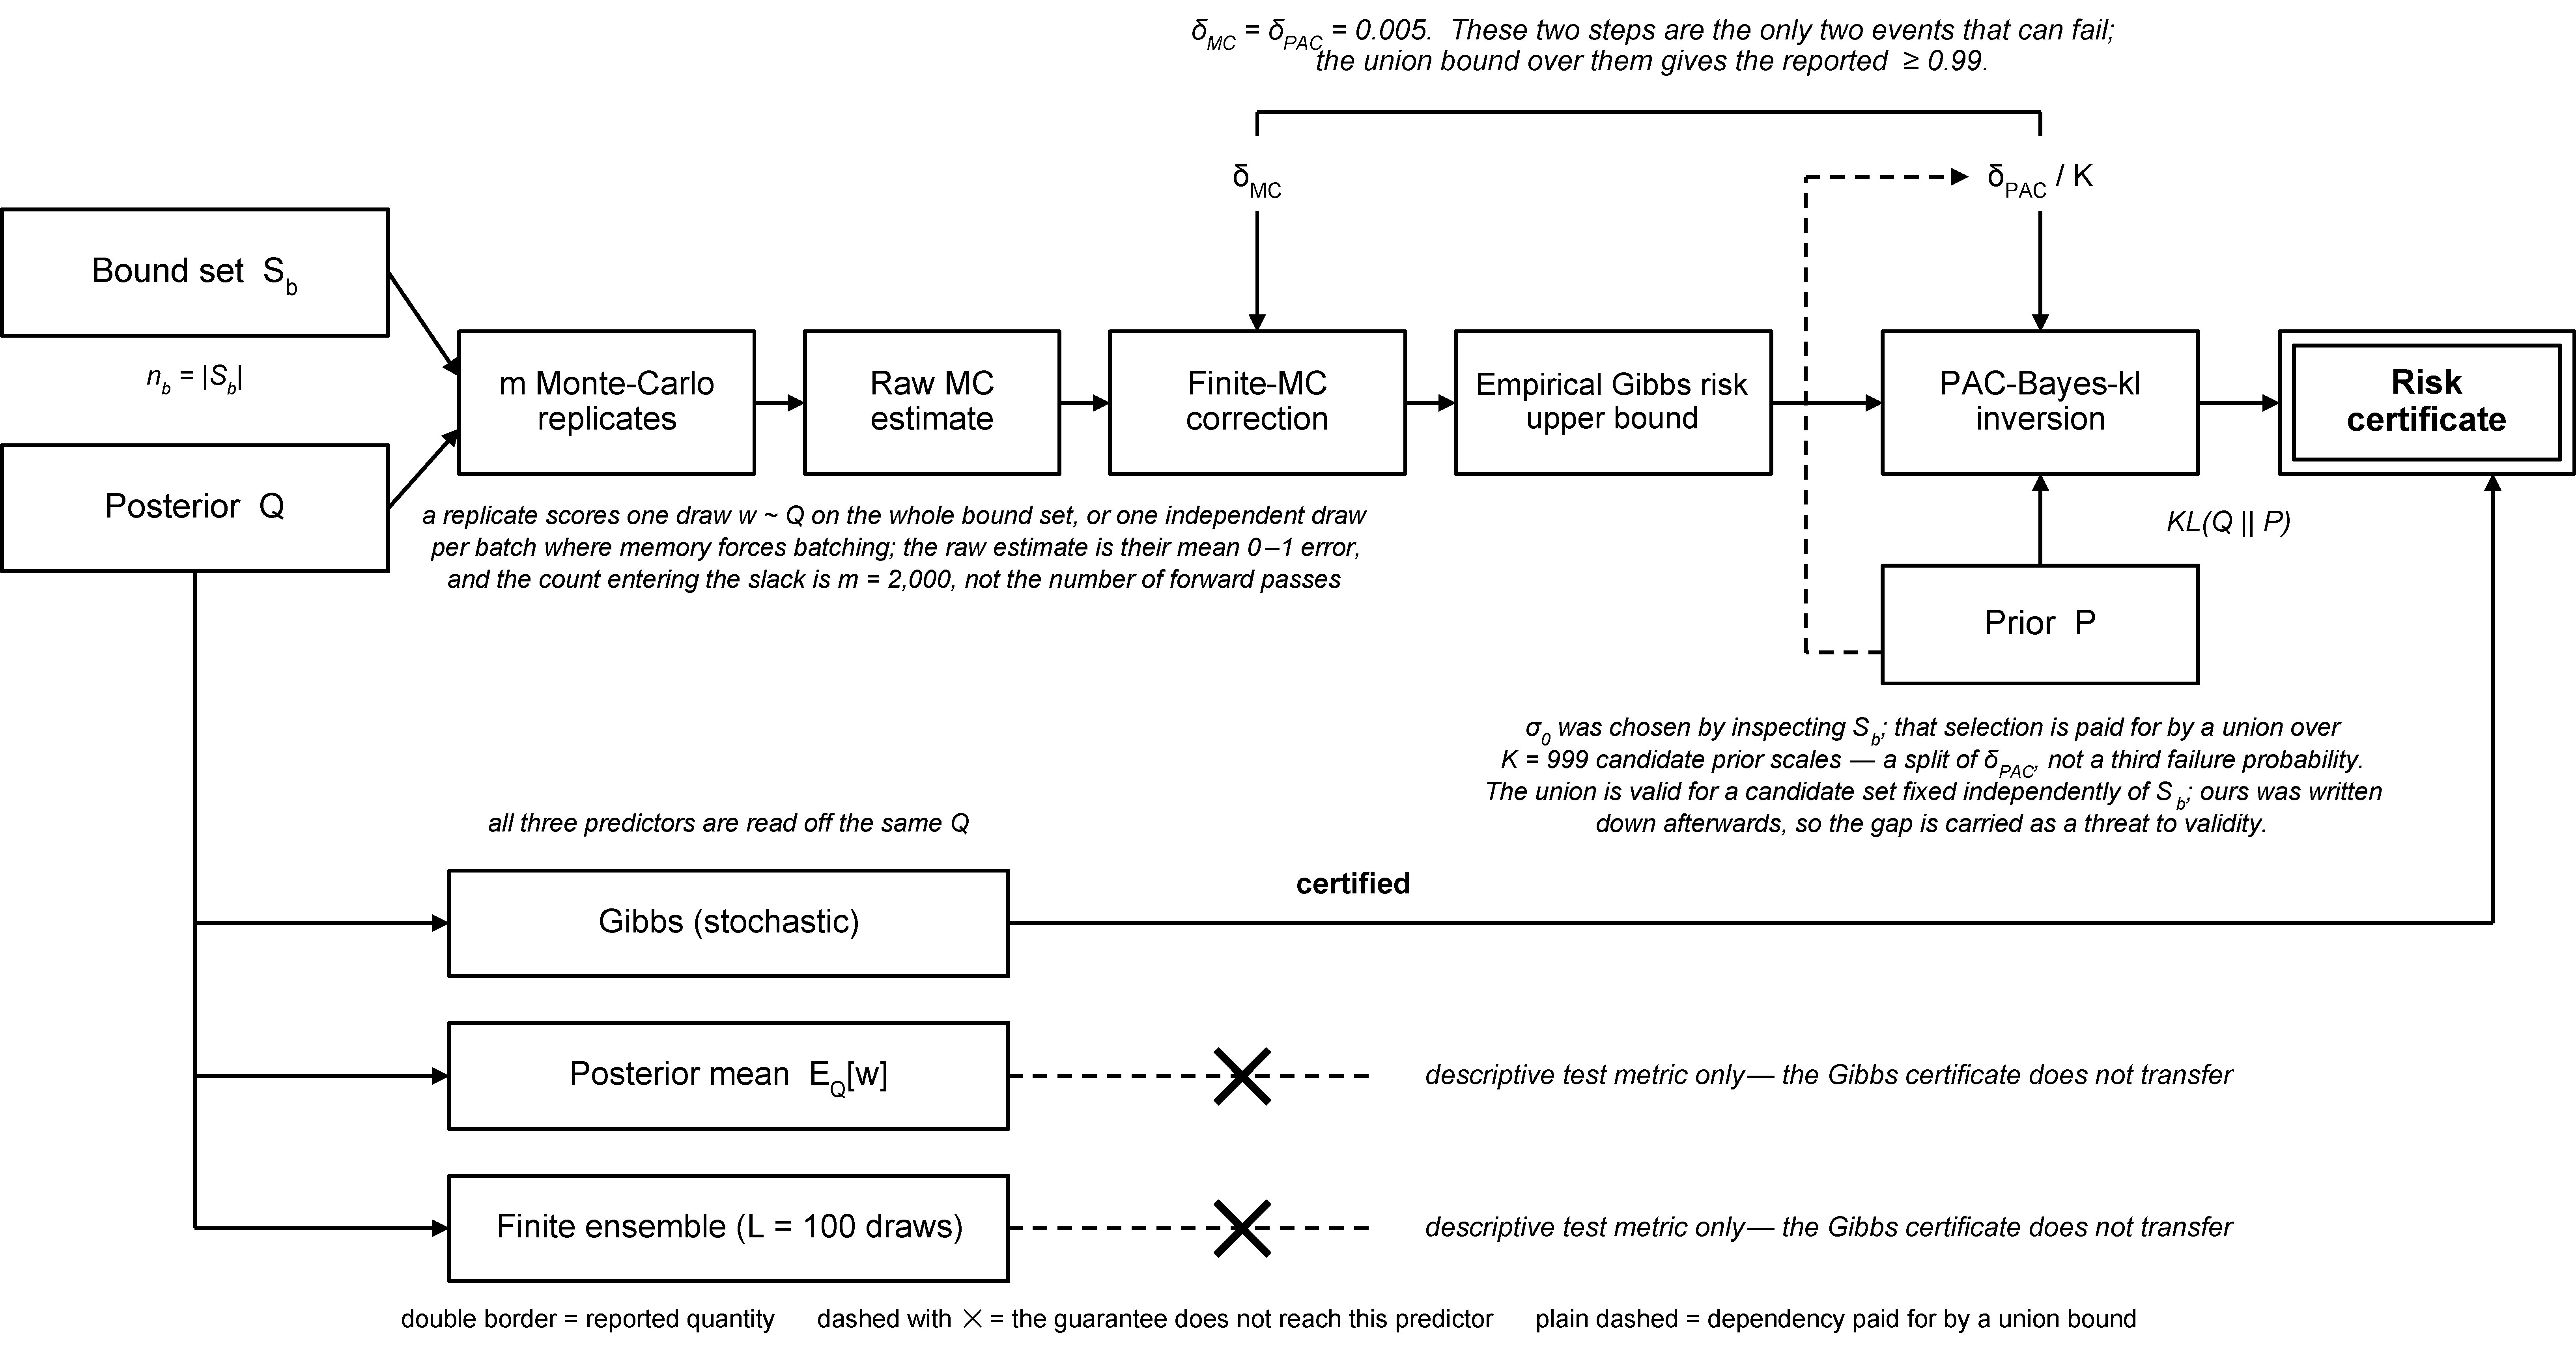
\includegraphics[width=\linewidth]{fig_certificate_chain.pdf}
\caption{The certificate computation, end to end. Two distinct corrections
stand between the raw Monte-Carlo estimate and the reported number, and the two
leader lines mark them as the only two events that can fail: their union is what
gives the $0.99$. The dashed branch from the prior records that $\sigma_0$ was
chosen by inspecting $S_{\mathrm b}$, which is paid for by splitting
$\delta_{\mathrm{PAC}}$ across the candidate grid rather than by a separate
failure probability. Bottom right: all three predictors come from the same $Q$,
but only the Gibbs one is certified, and the crossed lines mark that the
guarantee does not transfer to the other two.}\label{fig:chain}
\end{figure}

\paragraph{Choosing the prior spends part of the same budget.} The prior
scale $\sigma_0$ was not fixed in advance: it was settled after comparing
certificates computed on $S_{\mathrm b}$ (Section~\ref{sec:protocol}).
Inequality~\eqref{eq:pbkl} holds for a prior fixed independently of
$S_{\mathrm b}$, simultaneously over all posteriors; it does not licence
inspecting $S_{\mathrm b}$ and then picking one prior out of several for free.
The repair is one more union bound: applying~\eqref{eq:pbkl} to each of $K$
candidate priors at $\delta_{\mathrm{PAC}}/K$ makes the guarantee simultaneous
over all of them, so whichever is adopted is covered, at a cost of $\log K$ in
the numerator of the slack.

The obvious candidate set is the wrong one. Counting the scales we compared, the
three probed and the one adopted, gives $K=4$; but $0.03$ was picked \emph{after}
those curves were seen, so that set is itself a function of $S_{\mathrm b}$ and a
union over it covers nothing. We union instead over
$\Sigma=\{0.001,0.002,\dots,0.999\}$, every three-decimal scale in the unit
interval, so $K=999$. The price, $\log 999$ nats against $\log 4$, raises the
headline certificates by about $0.0005$ and the smallest bound set in the study,
the $10\%$-data cell at $n_{\mathrm b}=3{,}000$, by $0.004$; no comparison here
turns on that. We apply it to every cell, conservatively so for Fashion-MNIST and
CIFAR-10, whose bound sets were never consulted in choosing $\sigma_0$.

The union is
valid for any $\Sigma$ fixed independently of $S_{\mathrm b}$, and then covers the
adopted scale however it was picked from $\Sigma$. What we cannot show is that our
selection was confined to $\Sigma$ in advance: $\Sigma$ was written down
afterwards, and a procedure returning $0.0325$ would not have been covered. The
certificates therefore hold under the assumption that only a three-decimal scale
could have been produced, which we believe but cannot demonstrate from the
artefact. Pre-registration is one way to close that, but not the only one: it
would equally suffice to show the candidate set fixed in advance by the
configuration space or by the search procedure itself. Ours was not, so we carry
it as a threat to validity (Section~\ref{sec:threats}) rather than as a solved
problem.

The posterior needs no such treatment, since~\eqref{eq:pbkl} is already
simultaneous over all $Q$: the learning rate, the epoch count and everything else
shaping $Q$ may depend on the data freely. That licence covers the PAC-Bayes
event only, not the finite-Monte-Carlo step~\eqref{eq:mc}, which holds for the
$Q$ evaluated rather than simultaneously over candidates. Choosing a checkpoint
by comparing finite-$m$ certificates would therefore need its own correction; we
do not, computing each certificate once on the final-epoch posterior.

\subsection{Data partition: \texorpdfstring{$S$, $S_0$ and $S\setminus
S_0$}{S, S0 and S minus S0}}\label{sec:partition}

A learnt (data-dependent) prior is built by training on part of the data, which
is legitimate only if the bound set is kept independent of the prior. From the
full training set we
select a subset $S$, which is the whole training set unless we are studying data
scarcity. For a learnt prior we split $S$ into a \emph{prior subset}
$S_0\subset S$ (half of $S$) used to train the prior, and the disjoint \emph{bound
subset} $S_{\mathrm b}:=S\setminus S_0$ on which the empirical risk entering the
certificate is measured. The posterior $Q$ may be trained on all of $S$; the prior
$P$ depends only on $S_0$ and is therefore independent of $S_{\mathrm b}$,
as~\eqref{eq:pbkl} requires. Consequently
\begin{equation}\label{eq:counts}
n_{\mathrm{post}}=|S|,\qquad n_{\mathrm b}=|S_{\mathrm b}|.
\end{equation}
The second equality in~\eqref{eq:counts} is the one the audit of
Section~\ref{sec:pipeline} restores: it is the bound subset, not the dataset, that
supplies the denominator.
For a data-free (random) prior there is no $S_0$, the prior is independent of all
of $S$, and $n_{\mathrm b}=|S|$. On the full MNIST training set with an even
split this gives $n_{\mathrm{post}}=60{,}000$ and $n_{\mathrm b}=30{,}000$
($50{,}000$ and $25{,}000$ for CIFAR-10); putting $60{,}000$ in the denominator
instead, as a na\"ive reading of the partition suggests, understates the
complexity term and returns a certificate that is too tight. We therefore derive
$n_{\mathrm b}$ from explicit bound-subset membership and verify
$S_0\cap S_{\mathrm b}=\varnothing$ and $S_0\cup S_{\mathrm b}=S$ before
every run.

\begin{figure}[t]\centering
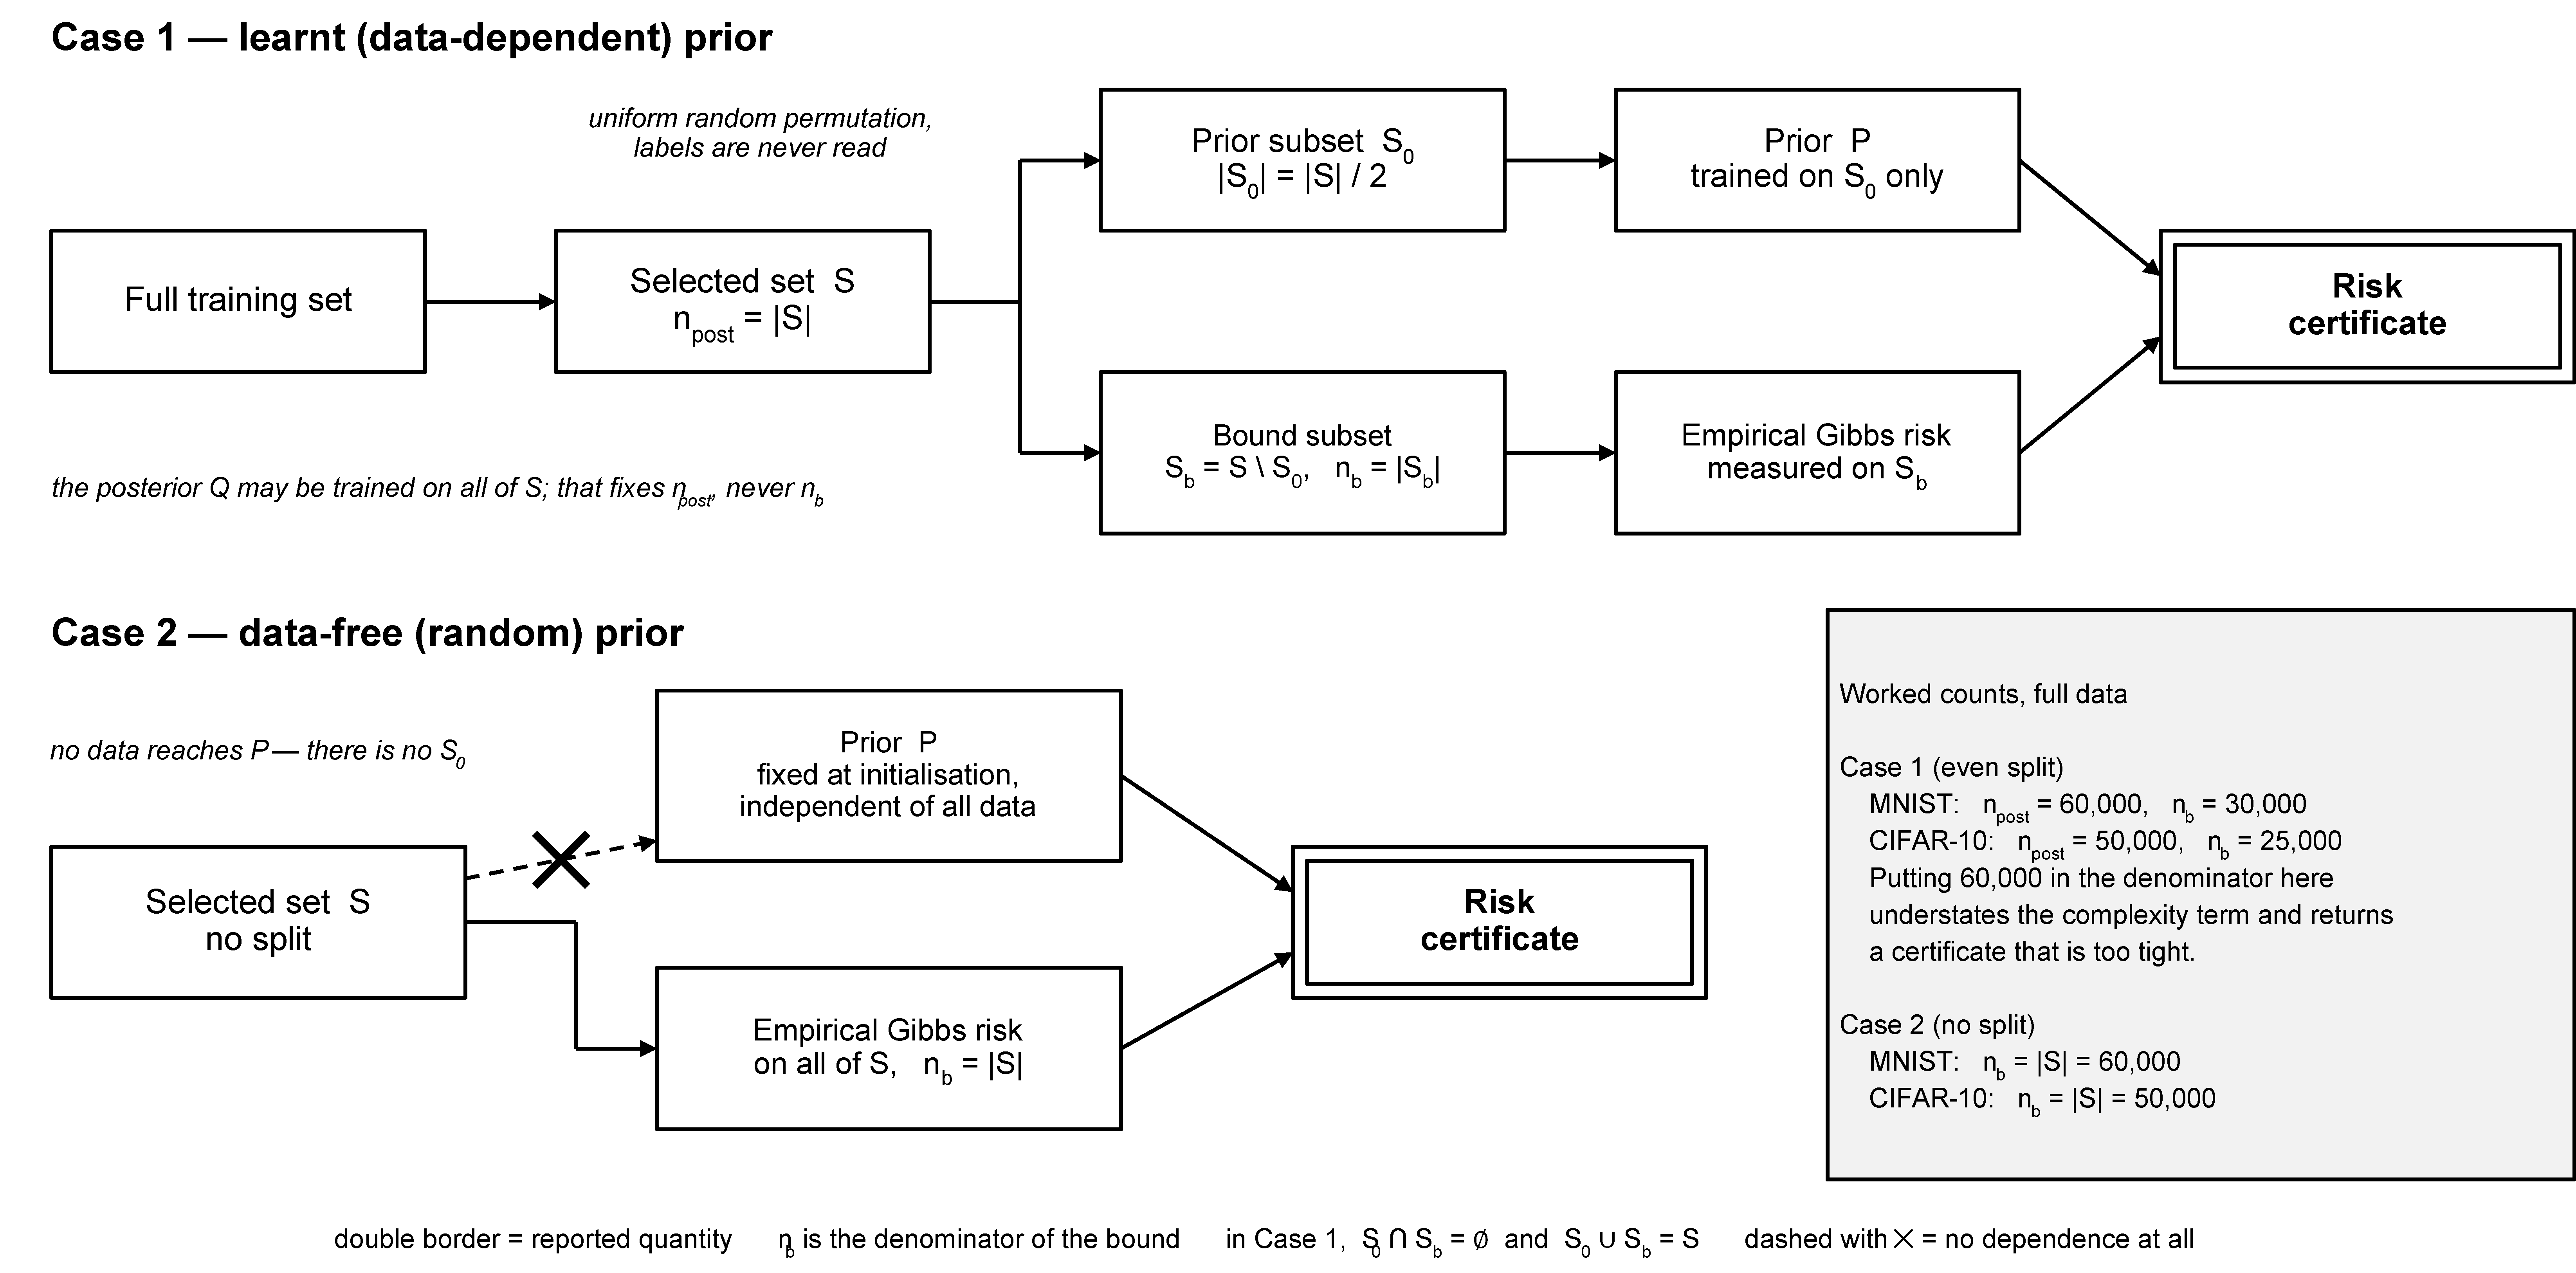
\includegraphics[width=\linewidth]{fig_partition.pdf}
\caption{Data partition and the two prior cases. A uniformly random subset $S$ is
drawn from the full training set, and in Case~1 split again into a prior subset
$S_0$ and a bound subset $S_{\mathrm b}=S\setminus S_0$. Both draws are made by
permutation alone and never read a label, which is what leaves $P$ admissible;
Figure~\ref{fig:flow} gives the dependence this buys. The certificate's
denominator is the size of whichever set the empirical risk is measured on, so it
is $n_{\mathrm b}=|S_{\mathrm b}|$ with a learnt prior and $n_{\mathrm b}=|S|$
with a data-free one --- the distinction the sample-count correction of
Section~\ref{sec:pipeline} restores.}\label{fig:partition}
\end{figure}

Figure~\ref{fig:partition} fixes which examples go where; what the bound
constrains is which subset may \emph{inform} which quantity
(Figure~\ref{fig:flow}).

\begin{figure}[t]\centering
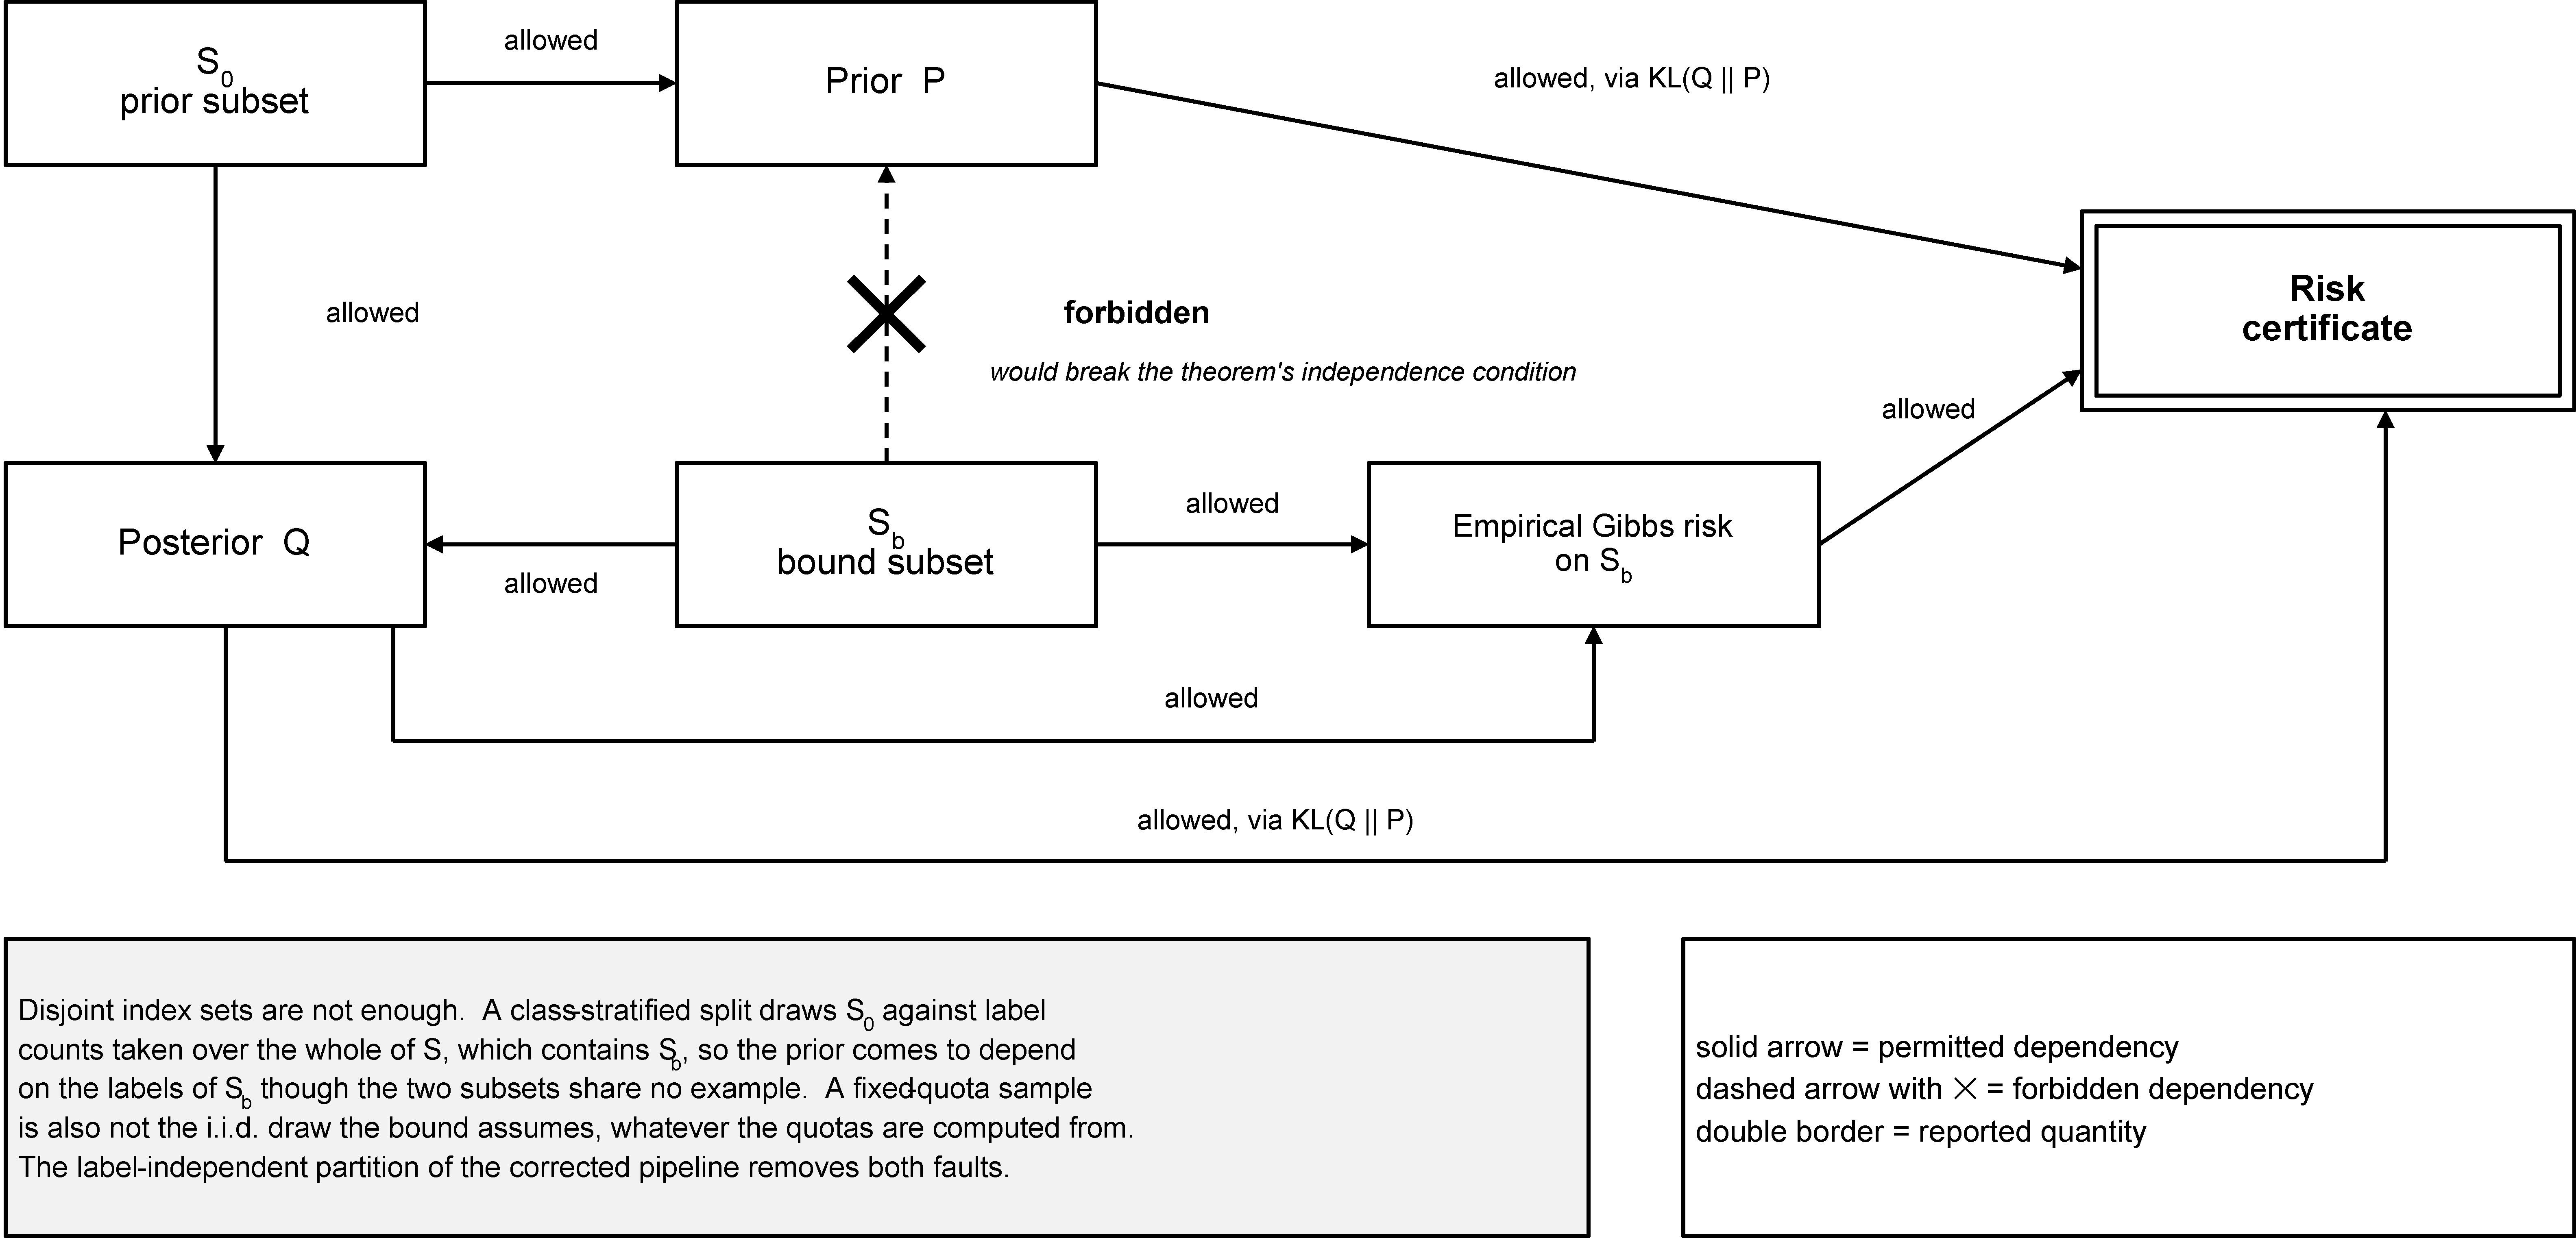
\includegraphics[width=0.92\linewidth]{fig_information_flow.pdf}
\caption{Permitted and forbidden information flow. The posterior may be informed
by every part of $S$; the prior may be informed only by $S_0$. The one forbidden
edge is $S_{\mathrm b}\to P$, and the note records why disjoint index sets are
not by themselves enough to rule it out: a class-stratified split sets $S_0$'s
quotas from label counts taken over all of $S$, so the prior can depend on the
bound set's labels without sharing a single example with it. That is the failure
the label-independent partition of Section~\ref{sec:pipeline}
removes.}\label{fig:flow}
\end{figure}

\subsection{Training objectives}\label{sec:objectives}

The posterior is trained by PAC-Bayes-with-Backprop \parencite{perezortiz2021}:
the weight distribution $Q$ (a diagonal Gaussian, mean and per-weight scale) is
optimised by gradient descent on a differentiable objective derived from a
PAC-Bayes bound, through the reparameterisation trick \parencite{blundell2015}.
Whether that objective is itself a bound depends on $\beta$, settled below. We compare three
bound-derived objectives and one accuracy-oriented baseline, all on
$n=n_{\mathrm{post}}$ training points with bounded empirical cross-entropy
$\hat{R}(Q)$ and confidence $\delta_{\mathrm{train}}$:
Writing $\kappa=\beta\,\mathrm{KL}(Q\|P)+\log\big(2\sqrt{n}/\delta_{\mathrm{train}}\big)$
for the complexity numerator shared by the first three:
\begin{itemize}
\item \textbf{$f_{\text{classic}}$} (McAllester/Pinsker):
  $f=\hat{R}(Q)+\sqrt{\kappa/(2n)}$.
\item \textbf{$f_{\lambda}$} \parencite{thiemann2017}: for a learnable
  $\lambda\in(0,2)$, optimised by alternating minimisation over $Q$ and $\lambda$,
  \[
  f=\frac{\hat{R}(Q)}{1-\lambda/2}+\frac{\kappa}{n\,\lambda\,(1-\lambda/2)}.
  \]
\item \textbf{$f_{\text{quad}}$}: the quadratic relaxation of PAC-Bayes-kl
  \parencite{perezortiz2021}, which with $\rho=\kappa/(2n)$ is
  \[
  f=\Big(\sqrt{\hat{R}(Q)+\rho}+\sqrt{\rho}\Big)^{2}.
  \]
  It is reported there as the tightest of the three with a data-dependent prior,
  though in our runs $f_{\text{classic}}$ is tighter (Section~\ref{sec:main}).
\item \textbf{$f_{\text{bbb}}$} (baseline): the Bayes-by-Backprop objective
  \parencite{blundell2015}, $f=\hat{R}(Q)+\beta\,\mathrm{KL}(Q\|P)/n$. It has the
  ELBO's form but is not the ELBO: $\hat{R}(Q)$ here is the clamped, rescaled
  cross-entropy of Section~\ref{sec:assumptions} rather than a log-likelihood, and
  $\beta<1$ down-weights the KL. It trades that KL against the empirical risk with
  a calibration that does not target the reported certificate, which is what makes
  it an accuracy-oriented control.
\end{itemize}
The KL penalty $\beta$ is carried by all four objectives, not only the baseline,
and following the reference's configuration we set $\beta=0.1$ throughout. This
makes each of the first three a down-weighted surrogate rather than the literal
bound it is named after, so the value each optimises is not itself a valid
certificate. That does not affect what we report, because the objective only
shapes $Q$: the reported certificate is always the \emph{same} PAC-Bayes-kl
inversion~\eqref{eq:invert} applied to the resulting $Q$, evaluated with the
unpenalised $\mathrm{KL}(Q\|P)$. No ordering of objectives by certificate value
is therefore fixed independently of the $Q$ they produce.

\subsection{Priors}\label{sec:priors}

We study two prior families. A \emph{data-free} (random) prior is a fixed
isotropic Gaussian at the initialisation, independent of all data: the most
distribution-independent choice, but one that typically leaves a large
$\mathrm{KL}(Q\|P)$ and a loose certificate. A \emph{data-dependent} (learnt)
prior centres $P$ at the weights of a network trained by empirical-risk
minimisation on $S_0$, with dropout to limit prior over-fitting, which moves $P$
close to well-performing posteriors and can sharply reduce the KL. The posterior
is initialised at the prior in both cases, and the legitimacy of the learnt one
rests on the independence of $P$ from $S\setminus S_0$
(Section~\ref{sec:partition}).

\section{Experimental Method}\label{sec:method}

\subsection{Datasets and preprocessing}\label{sec:datasets}

We use three standard image-classification benchmarks: \textbf{MNIST}
\parencite{lecun1998} (60{,}000 train / 10{,}000 test, $28\times28$ greyscale, 10
classes), \textbf{Fashion-MNIST} \parencite{xiao2017} (same shape, harder
classes), and \textbf{CIFAR-10} \parencite{krizhevsky2009} (50{,}000 / 10{,}000,
$32\times32$ colour, 10 classes). The only preprocessing is conversion to a
tensor and per-channel standardisation with the published training statistics:
mean $0.1307$ and standard deviation $0.3081$ for MNIST, $0.2860$ and
$0.3530$ for Fashion-MNIST, and $(0.4914,0.4822,0.4465)$ and
$(0.2023,0.1994,0.2010)$ for CIFAR-10, applied to train and test alike. We
avoid augmentation, resizing and pretraining so that the certificate reflects
the PAC-Bayes machinery rather than auxiliary engineering, and treat the
cross-dataset comparison as descriptive only, since architecture and compute
budget change across datasets (Section~\ref{sec:evaluation}).

\subsection{Architectures}\label{sec:arch}

Two families of probabilistic network are used, both carrying a diagonal-Gaussian
weight distribution with a mean and a per-weight scale for every parameter, so
that a probabilistic network holds twice as many parameters as its deterministic
counterpart (Table~\ref{tab:arch}). Every hidden activation is a ReLU, the output
is a log-softmax over the ten classes, and no batch normalisation, weight decay or
learning-rate schedule is used anywhere. Dropout appears only in the deterministic
network that builds a learnt prior, where it limits prior over-fitting to $S_0$;
the certified probabilistic networks have none, since the weight noise already
regularises them and a stochastic mask would add a second, uncertified source of
randomness to the Monte-Carlo estimate. The prior network shares the architecture
of its probabilistic counterpart, so its trained weights can initialise the prior
mean directly.

\begin{table}[h]\centering\small
\caption{Layer specifications of the five network variants used. Convolutions are written
as (input channels~$\to$~output channels, kernel, padding), and \texttt{MaxPool}
is $2\times2$ with stride $2$. Parameter counts are for the deterministic
network; the probabilistic counterpart carries twice as many, one mean and one
scale per weight.}\label{tab:arch}
\begin{tabular}{@{}l l r@{}}
\toprule
Network & Layers & Parameters \\
\midrule
FCN
  & $784\!\to\!600\!\to\!600\!\to\!600\!\to\!10$, fully connected
  & $1{,}198{,}210$ \\
(MNIST, Fashion-MNIST) & & \\[3pt]
CNN, 4 layers
  & \begin{tabular}[t]{@{}l@{}}
    Conv($1\!\to\!32$, $3\!\times\!3$, pad~$0$), Conv($32\!\to\!64$, $3\!\times\!3$, pad~$0$),\\
    MaxPool, flatten ($9216$), FC $9216\!\to\!128$, FC $128\!\to\!10$
    \end{tabular}
  & $1{,}199{,}882$ \\
(MNIST, Fashion-MNIST) & & \\[3pt]
CNN, 9 layers
  & \begin{tabular}[t]{@{}l@{}}
    Conv($3\!\to\!32$), Conv($32\!\to\!64$), MaxPool,\\
    Conv($64\!\to\!128$), Conv($128\!\to\!128$), MaxPool,\\
    Conv($128\!\to\!256$), Conv($256\!\to\!256$), MaxPool,\\
    flatten ($4096$), FC $4096\!\to\!1024\!\to\!512\!\to\!10$
    \end{tabular}
  & $5{,}851{,}338$ \\
(CIFAR-10) & & \\[3pt]
CNN, 13 layers
  & \begin{tabular}[t]{@{}l@{}}
    channels $32,64$ | $128,128$ | $256,256,256$ | $512,512,512$,\\
    MaxPool after each group; flatten ($2048$),\\
    FC $2048\!\to\!1024\!\to\!512\!\to\!10$
    \end{tabular}
  & $10{,}244{,}042$ \\
(CIFAR-10) & & \\[3pt]
CNN, 15 layers
  & \begin{tabular}[t]{@{}l@{}}
    channels $32,64$ | $128,128$ | $256,256,256,256$ | $512,512,512,512$,\\
    MaxPool after each group; flatten ($2048$),\\
    FC $2048\!\to\!1024\!\to\!512\!\to\!10$
    \end{tabular}
  & $13{,}193{,}930$ \\
(CIFAR-10) & & \\
\bottomrule
\end{tabular}

\smallskip
\footnotesize All convolutions are $3\!\times\!3$. The 4-layer network uses no
padding; the three CIFAR-10 networks pad by $1$. Dropout in the prior network is
channel-wise for the 4- and 9-layer architectures and element-wise for the 13-
and 15-layer ones; both follow the reference implementation, which differs
between them.
\end{table}

\subsection{Design choices}\label{sec:choices}

Every design choice prioritises analysing the certificate over maximising
accuracy. Four settle the study: every certificate is reported through the
PAC-Bayes-kl inversion \parencite{maurer2004,seeger2002}, the tightest of the
classical statements, so that the objectives differ only in the posterior they
produce; the learnt prior takes the disjoint-subset route rather than the
differential-privacy route of \textcite{dziugaite2018}, because its independence
condition is directly verifiable, at the cost of a smaller bound set; the
posterior is a diagonal Gaussian, which keeps the KL a sum of per-weight closed
forms; and the reference architectures are used without augmentation,
pretraining or a learning-rate schedule. The departures from the reference are
compute-driven rather than chosen: a per-cell grid search of its size, over
five seeds, three datasets and five architectures, is beyond the compute here, so
we fix one configuration and take a smaller Monte-Carlo budget, then measure that
budget rather than assume it (Section~\ref{sec:mc}). Appendix~\ref{app:choices}
gives the alternatives considered and rejected in each case.

\subsection{Corrected pipeline}\label{sec:pipeline}

All experiments use a clean reimplementation that makes the certificate
bookkeeping explicit and testable. It makes five tested changes to the reference
pipeline, three of which alter the reported certificate value.
Figure~\ref{fig:audit} places each on the stage it acts on.

\begin{figure}[t]\centering
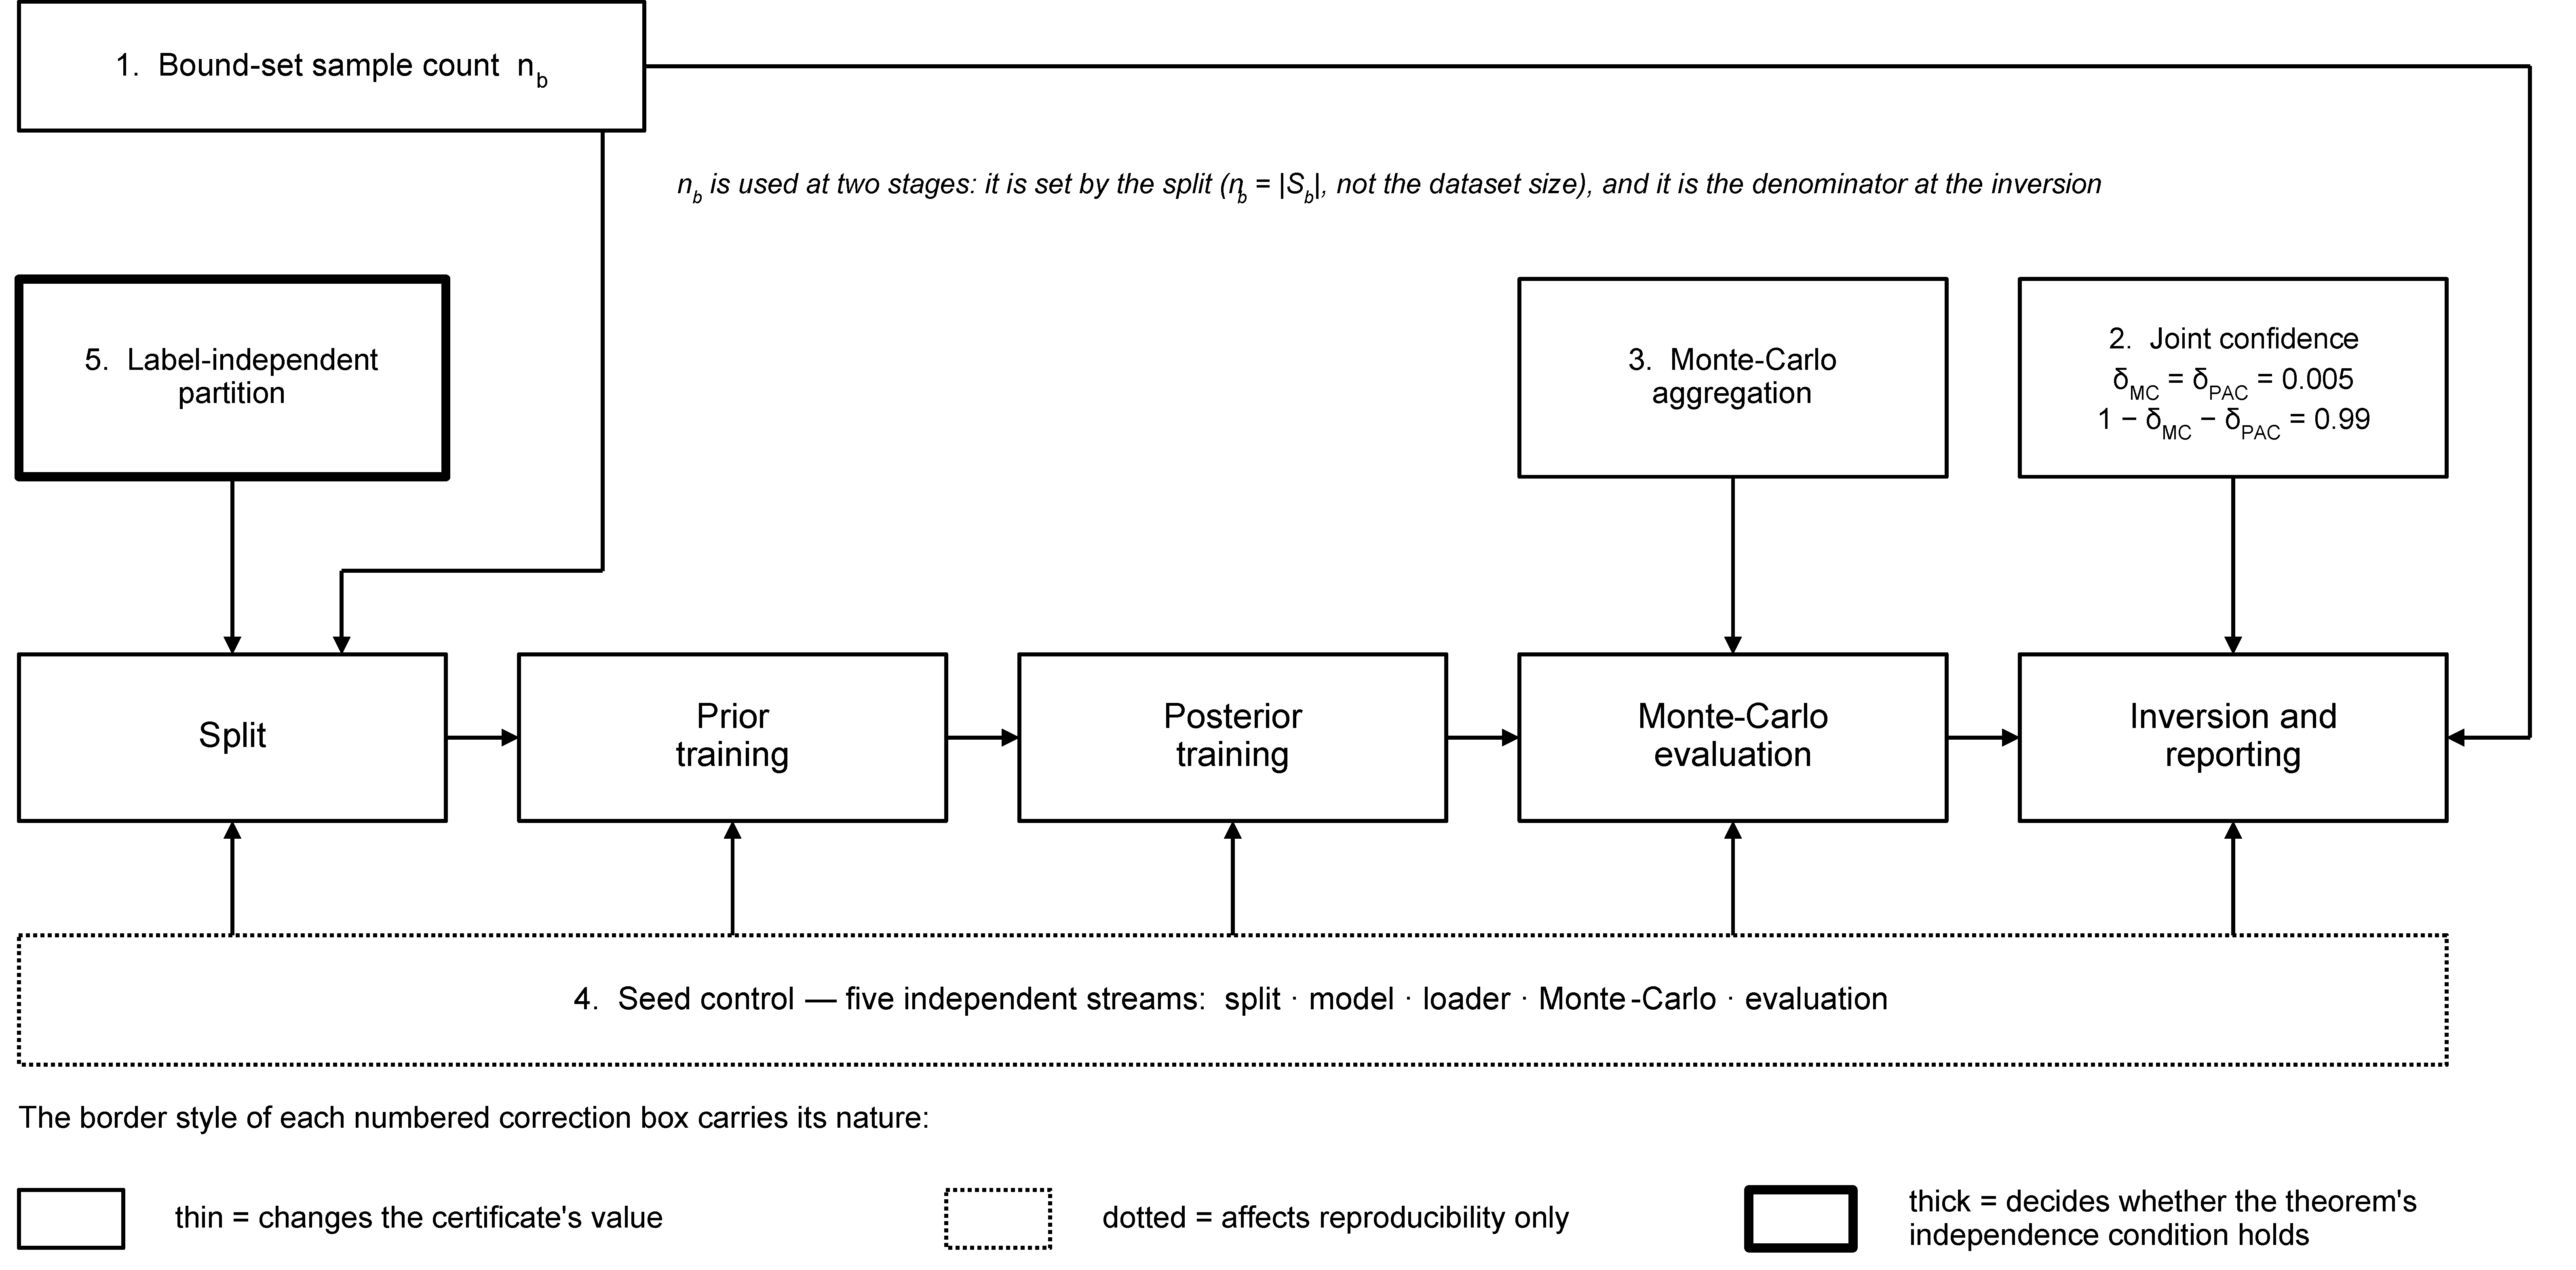
\includegraphics[width=\linewidth]{fig_audit_map.pdf}
\caption{Where each correction acts. The border style carries the distinction
the list cannot: three change the certificate's value, one affects only
reproducibility, and one decides whether the theorem's independence condition
holds at all. The sample count is drawn against two stages because it is used at
both, entering the split and again the inversion that reports the
bound.}\label{fig:audit}
\end{figure}
\begin{enumerate}
\item \textbf{Bound-set sample count.} The denominator $n_{\mathrm b}$
  in~\eqref{eq:pbkl} is $|S_{\mathrm b}|$, the held-out bound subset, not the
  size of the underlying dataset.
\item \textbf{Joint confidence.} The Monte-Carlo and PAC-Bayes steps use separate
  failure probabilities $\delta_{\mathrm{MC}}=\delta_{\mathrm{PAC}}=0.005$,
  combined by a union bound to a reported confidence of $0.99$, rather than reusing
  one $\delta$ across both inversions.
\item \textbf{Monte-Carlo aggregation.} The empirical Gibbs risk is accumulated
  example-weighted over the bound set and averaged over exactly $m$ samples,
  fixing an off-by-one in the original per-batch averaging.
\end{enumerate}
The fourth affects reproducibility; the fifth affects whether the learnt-prior
construction satisfies the theorem's independence condition at all, though
neither changes the certificate arithmetic once the split is fixed:
\begin{enumerate}\setcounter{enumi}{3}
\item \textbf{Seed control.} Five independent seed streams (split, model, loader,
  Monte-Carlo, evaluation) are derived from one base seed, so the seed genuinely
  changes the split and the model. The evaluation stream is separate so that the
  descriptive test errors, which also sample posterior weights, do not inherit
  the RNG state the certificate's $m$ draws left behind: otherwise raising the
  Monte-Carlo budget would move a test error that does not depend on it.
\item \textbf{Label-independent partition.} The subset $S$ and its split into
  $S_0$ and $S_{\mathrm b}$ are drawn by a uniform random permutation rather than
  by taking a prefix. We first replaced the prefix split with a class-stratified
  one, then rejected that. Its class quotas are taken over the whole of $S$, which
  contains $S_{\mathrm b}$, so $S_0$ comes to depend on bound-set labels; and a
  sample with fixed class quotas is not the i.i.d.\ draw the bound assumes.
\end{enumerate}
All five rest on the explicit, saved bookkeeping of
Section~\ref{sec:compute}, which also keeps the six notions of error distinct:
the raw Monte-Carlo $0$--$1$ estimate, the corrected empirical Gibbs risk, the
certificate, and the stochastic, posterior-mean and ensemble test errors, so the
certified quantity is never silently conflated with a test error.

Each test targets a specific correction rather than basic pipeline execution, and
fixes a concrete input and an expected output rather than a plausible range: the
split tests assert the counts $6{,}000$ and $3{,}000$ at a tenth of the data, the
aggregation test asserts agreement to $10^{-9}$ between a single batch and a
ragged batching of a deterministic posterior, and the confidence test asserts
$0.99$ to $10^{-12}$ rather than $1-\delta$. Appendix~\ref{app:tests} lists all
forty-two with their tolerances.
A test that never fails defends nothing, so we checked that each bites rather
than assuming it: disabling the prior-selection union in the source makes two of
its five tests fail, and letting one $S_0$ example into the bound loader makes
two of the loader tests fail. They check the bookkeeping around the bound, not the bound itself.

\subsection{Training protocol}\label{sec:protocol}

Both the prior network and the posterior are trained by SGD with momentum and no
weight decay. The prior network minimises the negative log-likelihood of its
labels on $S_0$; the posterior minimises the objective of
Section~\ref{sec:objectives}. Table~\ref{tab:hparams} lists every setting, and one training configuration is
shared by every cell: its entries do
not vary with the dataset, the architecture, the objective or the prior family.
Only the evaluation batch cap differs, and for memory rather than training
reasons: the bound set is scored in a single batch for the FCN cells, in batches
of $2{,}500$ for the two CNN cells on $28\times28$ data, and $12{,}500$ on
CIFAR-10, so that the deeper networks' Monte-Carlo evaluation fits in device
memory. The cap changes how the estimate is batched, not what it estimates
(Section~\ref{sec:confidence}).

\begin{table}[h]\centering\small
\caption{The training configuration shared by every cell.}\label{tab:hparams}
\begin{tabular}{@{}llll@{}}
\toprule
Optimiser & SGD, no weight decay & Prior scale $\sigma_0$ & $0.03$ \\
Posterior learning rate & $5\times10^{-3}$ & Prior distribution & Gaussian \\
Posterior momentum & $0.95$ & $p_{\min}$ & $10^{-5}$ \\
Prior learning rate & $5\times10^{-3}$ & $\delta_{\mathrm{train}}$ & $0.025$ \\
Prior momentum & $0.99$ & $\delta_{\mathrm{MC}}$, $\delta_{\mathrm{PAC}}$ & $0.005$ each \\
Prior dropout & $0.2$ & Monte-Carlo samples $m$ & $2{,}000$ \\
Batch size & $250$ & Ensemble samples $L$ & $100$ \\
Prior epochs & $70$ & Prior/bound split & $0.5$ \\
Posterior epochs & $100$ & KL penalty $\beta$ (all objectives) & $0.1$ \\
\bottomrule
\end{tabular}
\end{table}

Since one fixed configuration replaces the reference's per-cell grid search, two
of these values were not simply copied.
The learning rates, momenta, $\sigma_0$, $p_{\min}$, batch size and
$\delta_{\mathrm{train}}$ are those the reference reports for MNIST, and the epoch
counts follow its statement that the networks converge by roughly $70$ epochs. One
value had to be recovered rather than copied: the reference implementation's
example script ships a posterior learning rate of $10^{-3}$, at which our first
grid gave a stochastic test error about four times the published one, whereas the
reference's text identifies $10^{-3}$ as converging slowly and $5\times10^{-3}$ as
the working value. We resolved that in favour of the text, but what prompted us
to look was a test-set discrepancy, so the learning-rate choice was indirectly
informed by the test set. It costs the certificate nothing, since it acts only on
the posterior, but it does mean the reported test errors are not a wholly
untouched estimate. Apart from that, the only sweep we ran ourselves was over the prior scale,
$\sigma_0\in\{0.01,0.02,0.05\}$ on MNIST at a reduced budget: the certificate was
almost unchanged across $[0.02,0.05]$ and degraded at $0.01$, so $\sigma_0=0.03$
sits in a flat region rather than at a tuned optimum. Those comparisons read
certificates computed on the bound set, so the prior was selected using
$S_{\mathrm b}$, and every certificate we report is corrected for that by the
union of Section~\ref{sec:confidence}. The reference grid-searches the same
parameter per cell without any such correction. This remains an explicitly
\emph{reduced-compute protocol}: the reference grid-searches learning rate, prior
scale and dropout per cell. Section~\ref{sec:mc} measures the effect of the
smaller $m$; the absent grid search is not quantified and is carried as a threat
to validity (Section~\ref{sec:evaluation}).

\subsection{Seeds and statistics}\label{sec:seeds}

Each headline cell is run over five base seeds ($0$--$4$), each genuinely
changing the data split, the model initialisation, the loader order and the
Monte-Carlo draws. Main-table quantities are means~$\pm$~standard deviations over
seeds, with per-seed values in the appendix. The across-seed variability of the
training procedure is not a PAC-Bayes confidence interval.

\subsection{Sensitivity and controlled-difficulty studies}\label{sec:studies}

Three further studies use the saved checkpoints. The \textbf{Monte-Carlo
sensitivity} curve isolates the effect of the sample budget $m$ on a fixed
posterior. At each budget
$m\in\{1{,}000,2{,}000,5{,}000,10{,}000,50{,}000,150{,}000\}$, up to the
reference's, we genuinely re-draw the Monte-Carlo estimate on the checkpoint and
recompute the certificate. Since the raw mean is an unbiased estimate of the
Gibbs risk, the only systematic route by which $m$ enters is the finite-MC slack
$\log(2/\delta_{\mathrm{MC}})/m$ of the first KL inversion, so we also compute an
analytical curve with the estimate held at its $m=1{,}000$ value; the two
agreeing is what shows the movement is slack and not a shifting estimate. The \textbf{small-data} sweep retrains the MNIST
FCN $f_{\text{quad}}$ learnt-prior cell on $100$, $50$, $20$ and $10\%$ of the
training data, with the corrected $n_{\mathrm b}$. The \textbf{controlled-difficulty} study
applies label noise $\eta\in\{0,0.1,0.2,0.4\}$ to the same cell with
architecture, sample size and compute held fixed.

The noise is symmetric: each example of $S$ is independently marked with
probability $\eta$ and a marked label is replaced by one drawn uniformly from the
nine \emph{other} classes, so a corrupted label is never the original and the
expected fraction of wrong labels is $\eta$. It is applied once, to $S$ as a whole
and before the prior/bound split, so $S_0$ and $S_{\mathrm b}$ are corrupted at
the same rate and the prior network also trains on noisy labels; the test set is
untouched, and the noise draw has its own seed. The certificate then bounds the
Gibbs risk under the
noisy-label distribution, whereas the test errors in the same rows are measured
against clean labels, so the two are not comparable. All three studies use the
same five seeds as the headline matrix.

\subsection{Compute and reproducibility}\label{sec:compute}

Experiments run on two NVIDIA RTX 3080 cards (20\,GB each) under PyTorch 2.5.1
and CUDA 12.4 \parencite{paszke2019}, and the full study comprises $115$ runs. Results are
aggregated from the per-run records into a single processed registry, which
de-duplicates by the full configuration and records the status and any exclusion
reason of every run, so that failed or non-finite runs are dropped with a stated
reason rather than silently. One criterion beyond the mechanical ones is the only
exclusion any run triggers. A
learnt-prior cell whose prior network never leaves the chance-level plateau is
not an instance of the protocol, since the posterior is then initialised at an
untrained prior, so we exclude a learnt-prior run whose prior network finishes
within five percentage points of chance, which for ten classes is $0.90$, on
$S_0$, the subset it was trained on. Scoring the screen there rather than on the
test set keeps it a training diagnostic: it consults no held-out data and exists
before any certificate does, so it cannot be tuned against a result. Separation
is wide: prior networks that trained reach at most $0.228$ on $S_0$, and the two
that did not sit at $0.866$ and $0.899$. Every table and figure reporting
experimental results in this dissertation is produced from that registry;
Figures~\ref{fig:chain}--\ref{fig:audit} are explanatory schematics rather than
results figures, and the pre-correction outputs are retained separately as an
archival audit record and are not used in any reported result.

This provenance is what allows each reported certificate to be recomputed and
checked independently. Each run stores all of its
seeds, the sample accounting ($n_{\mathrm{total}}$, $n_{\mathrm{selected}}$,
$n_{\mathrm{prior}}$, $n_{\mathrm{posterior}}$, $n_{\mathrm b}$), the three
confidence parameters, the raw Monte-Carlo estimate, the KL and the resulting
certificate, alongside the library versions, the hardware and the software version.
Any certificate can therefore be recomputed without re-training, which is how the
prior-selection union of Section~\ref{sec:confidence} was applied to all runs
after the fact. The registry carries the corrected and uncorrected values side by
side, and recomputing
the uncorrected column from the stored ingredients reproduces all $115$ recorded
certificates to $10^{-9}$.

The artefact is laid out so that each of those claims can be checked from a
command. One YAML file per headline cell fixes every entry of
Table~\ref{tab:hparams}, and the published values used in Table~\ref{tab:repro}
are held in a separate reference file annotated with the source column each was
read from, so the comparison cannot drift onto a different column of the
reference table. Appendix~\ref{app:repro} gives the directory layout, the
commands that regenerate a run, the matrix, the tests and every derived output,
and the pinned environment.

\section{Results}\label{sec:results}

All tables and figures below are generated from the processed results registry,
as are the values quoted in the running text.

\subsection{Correctness checks}\label{sec:correctness}

All forty-two tests of Appendix~\ref{app:tests} pass, and three checks run over
the results themselves. Every certificate recomputes from its saved Monte-Carlo
estimate, KL and $n_{\mathrm b}$, reproducing all $115$ recorded values to
$10^{-9}$, and this now gates aggregation. Every saved partition recomputes from
its recorded seed and matches index for index, so no reported run used a
label-dependent split whatever its configuration says. And each run asserts
before training that its loaders carry that partition, so the indices checked are
the indices consumed. Each reported $0.99$ confidence is \emph{per certificate,
per run}: a mean over seeds describes several such certificates and is not
itself a $0.99$ bound, which would need a further union over the rows. It is
conditional in one further respect, stated in Section~\ref{sec:confidence}: the
union over prior scales assumes a candidate grid fixed independently of the
bound set, which we argue for but cannot demonstrate. Every $0.99$ below carries
that assumption.

\subsection{Reproduction and main results}\label{sec:main}

\begin{sidewaystable}\centering
\caption{Headline cells (mean~$\pm$~SD over five seeds). Each run's certificate is
a $0$--$1$ PAC-Bayes-kl bound on the Gibbs risk holding at confidence $0.99$; the
column is the descriptive mean of five such per-run certificates and is not
itself a $0.99$ bound, which would need a further union over the five. The two
test errors are descriptive deployment metrics and carry no guarantee.
$n_{\mathrm b}$ is the bound-set size actually used, which halves for a learnt
prior.}\label{tab:main}
\begin{tabular}{llll r r r r r r}
\toprule
Dataset & Model & Prior & Obj. & $n_{\text{bound}}$ & Emp.\ Gibbs & KL$/n_{\text{bound}}$ & \textbf{Certificate} & Gibbs test & Post.mean test \\
\midrule
CIFAR-10 & CNN & learnt & $f_{\text{bbb}}$ & 25000 & $0.0767\pm0.0027$ & $3.35041$ & $0.9801\pm0.0024$ & $0.2412\pm0.0103$ & $0.2162\pm0.0054$ \\
CIFAR-10 & CNN & learnt & $f_{\text{classic}}$ & 25000 & $0.3174\pm0.0086$ & $0.01169$ & $0.3932\pm0.0084$ & $0.2902\pm0.0091$ & $0.2615\pm0.0077$ \\
CIFAR-10 & CNN & learnt & $f_{\text{quad}}$ & 25000 & $0.3003\pm0.0084$ & $0.03373$ & $0.4277\pm0.0074$ & $0.2802\pm0.0086$ & $0.2525\pm0.0077$ \\
CIFAR-10 & CNN & data-free & $f_{\text{quad}}$ & 50000 & $0.9203\pm0.0006$ & $0.00029$ & $0.9297\pm0.0005$ & $0.8978\pm0.0020$ & $0.9000\pm0.0000$ \\
CIFAR-10 & cnn13 & learnt & $f_{\text{quad}}$ & 25000 & $0.2416\pm0.0033$ & $0.04760$ & $0.3881\pm0.0038$ & $0.2202\pm0.0055$ & $0.1791\pm0.0027$ \\
CIFAR-10 & cnn15 & learnt & $f_{\text{quad}}$ & 25000 & $0.3134\pm0.0524$ & $0.05188$ & $0.4722\pm0.0487$ & $0.2847\pm0.0462$ & $0.2265\pm0.0459$ \\
Fashion-MNIST & CNN & learnt & $f_{\text{quad}}$ & 30000 & $0.1069\pm0.0014$ & $0.01411$ & $0.1674\pm0.0048$ & $0.0931\pm0.0024$ & $0.0866\pm0.0011$ \\
Fashion-MNIST & FCN & learnt & $f_{\text{bbb}}$ & 30000 & $0.0913\pm0.0007$ & $0.72021$ & $0.6632\pm0.0045$ & $0.1118\pm0.0016$ & $0.1018\pm0.0017$ \\
Fashion-MNIST & FCN & learnt & $f_{\text{classic}}$ & 30000 & $0.1387\pm0.0013$ & $0.00087$ & $0.1582\pm0.0017$ & $0.1204\pm0.0028$ & $0.1136\pm0.0024$ \\
Fashion-MNIST & FCN & learnt & $f_{\text{quad}}$ & 30000 & $0.1349\pm0.0011$ & $0.00526$ & $0.1746\pm0.0024$ & $0.1186\pm0.0030$ & $0.1109\pm0.0035$ \\
Fashion-MNIST & FCN & data-free & $f_{\text{quad}}$ & 60000 & $0.2461\pm0.0018$ & $0.08728$ & $0.4480\pm0.0011$ & $0.2254\pm0.0062$ & $0.1891\pm0.0056$ \\
MNIST & CNN & learnt & $f_{\text{quad}}$ & 30000 & $0.0201\pm0.0006$ & $0.00414$ & $0.0369\pm0.0013$ & $0.0108\pm0.0011$ & $0.0095\pm0.0009$ \\
MNIST & FCN & learnt & $f_{\text{bbb}}$ & 30000 & $0.0138\pm0.0003$ & $0.24945$ & $0.2658\pm0.0065$ & $0.0187\pm0.0007$ & $0.0149\pm0.0006$ \\
MNIST & FCN & learnt & $f_{\text{classic}}$ & 30000 & $0.0373\pm0.0006$ & $0.00022$ & $0.0455\pm0.0008$ & $0.0240\pm0.0009$ & $0.0192\pm0.0010$ \\
MNIST & FCN & learnt & $f_{\lambda}$ & 30000 & $0.0294\pm0.0005$ & $0.02032$ & $0.0777\pm0.0013$ & $0.0211\pm0.0003$ & $0.0170\pm0.0005$ \\
MNIST & FCN & learnt & $f_{\text{quad}}$ & 30000 & $0.0328\pm0.0006$ & $0.00625$ & $0.0580\pm0.0011$ & $0.0219\pm0.0006$ & $0.0176\pm0.0003$ \\
MNIST & FCN & data-free & $f_{\text{quad}}$ & 60000 & $0.1199\pm0.0020$ & $0.13763$ & $0.3496\pm0.0028$ & $0.0927\pm0.0033$ & $0.0570\pm0.0018$ \\
\bottomrule
\end{tabular}

\end{sidewaystable}

\begin{figure}[h]\centering
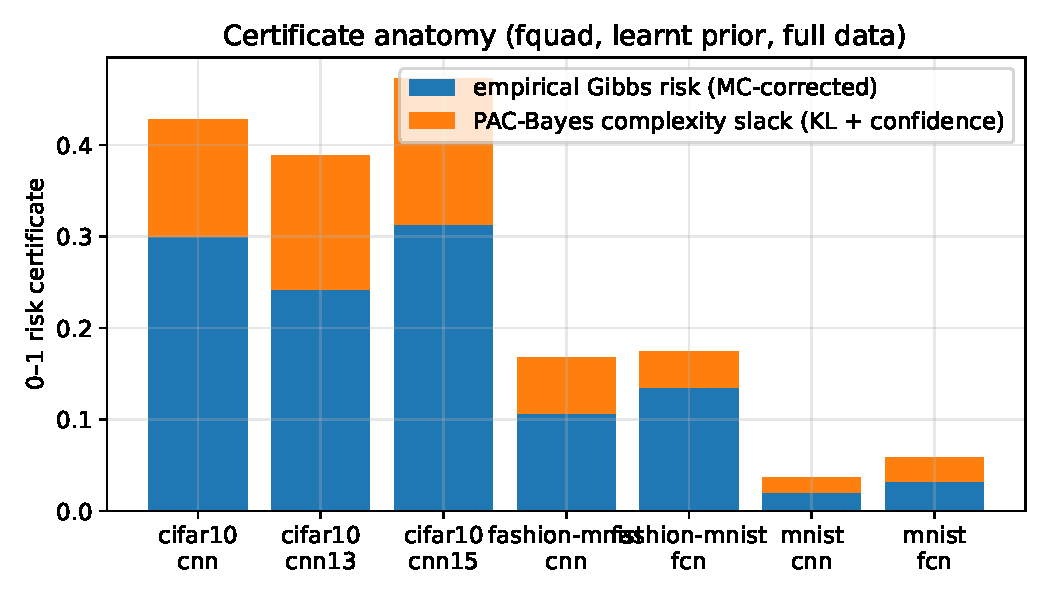
\includegraphics[width=0.8\linewidth]{fig_certificate_anatomy.pdf}
\caption{Certificate anatomy: the empirical Gibbs risk and the PAC-Bayes
complexity slack (KL + confidence terms) for the learnt-prior $f_{\text{quad}}$
cells.}\label{fig:anatomy}
\end{figure}

On MNIST with a learnt prior, the tightest $0$--$1$ certificate is obtained by
$f_{\text{classic}}$ ($\CertMnistFcnFclassicLearnt$), followed by $f_{\text{quad}}$
($\CertMnistFcnFquadLearnt$), $f_{\lambda}$ ($\CertMnistFcnFlambLearnt$) and
$f_{\text{bbb}}$ ($\CertMnistFcnBbbLearnt$); all are non-vacuous and reproduce the
qualitative finding of the reference that bound-minimising objectives yield far
tighter certificates than the accuracy-oriented $f_{\text{bbb}}$ baseline, whose
certificate is loose precisely because it carries the largest KL term
(Table~\ref{tab:main}). We do \emph{not} observe the
$f_{\text{quad}}\lesssim f_{\lambda}<f_{\text{classic}}$ ordering sometimes
quoted: the certificate is the same PAC-Bayes-kl inversion for every objective, so
the ordering reflects only which posterior each produces, and here
$f_{\text{classic}}$ yields the lowest-KL one. With the hyper-parameters fixed
this is a comparison of these runs, not a general ordering of the objectives.
Consistently, $f_{\text{bbb}}$ attains the best stochastic test error on MNIST
($\StochMnistFcnBbbLearnt$ against $\StochMnistFcnFquadLearnt$ for $f_{\text{quad}}$)
yet the loosest certificate, because its objective is not calibrated to the
reported bound.

Figure~\ref{fig:anatomy} shows where the looseness comes from. For the tight
learnt-prior cells the certificate sits only a little above the
empirical Gibbs risk: on the MNIST FCN $f_{\text{classic}}$ cell the complexity slack
$\mathrm{KL}/n_{\mathrm b}$ is around $0.0002$, so the bound is almost entirely
empirical risk. As the posterior is allowed a larger KL the slack grows:
$f_{\text{quad}}$ and $f_{\lambda}$ trade slightly lower empirical risk for a
noticeably larger KL, which is why they come out looser than $f_{\text{classic}}$
at similar accuracy, and $f_{\text{bbb}}$ is the extreme, its KL dominating the
certificate even though its empirical risk is the smallest of the four.
Tightness therefore depends on the empirical risk and on the KL cost of reaching
it, not on accuracy alone. That also explains the cross-dataset behaviour: the
empirical-risk floor rises with difficulty (Section~\ref{sec:erroranalysis} shows
where), so even a well-controlled KL cannot pull Fashion-MNIST or CIFAR-10 into
the MNIST range.

\paragraph{Comparison with the published numbers.} Table~\ref{tab:repro} sets our
values against the reference's for the four MNIST cells named as reproduction
targets in Section~\ref{sec:rqs}, using the same-definition columns recorded in
the reference file of Section~\ref{sec:compute}. All four reproduce on the
test-error metric: the stochastic test error differs from the published value by
between $\ReproStochDeltaMin$ and $\ReproStochDeltaMax$, inside the
one-percentage-point tolerance, and
the sign of the difference varies between cells rather than pointing one way, as
it would if our posteriors were systematically better or worse trained. That is
evidence about predictive behaviour, not about each component: the test error is
end-to-end, and the component claims rest on the tests of
Appendix~\ref{app:tests}.

\begin{table}[h]\centering\small
\caption{Reproduction of the four MNIST cells named in Section~\ref{sec:rqs},
against the published values of \textcite{perezortiz2021}. Ours are means over
five seeds. The published numbers were obtained with $m=150{,}000$ Monte-Carlo
samples and a per-cell grid search; ours with $m=2{,}000$ and one fixed
configuration.}\label{tab:repro}
\begin{tabular}{@{}lll rr r rr r@{}}
\toprule
& & & \multicolumn{3}{c}{Certificate} & \multicolumn{3}{c}{Stochastic test error} \\
\cmidrule(lr){4-6}\cmidrule(lr){7-9}
Model & Prior & Obj. & Published & Ours & $\Delta$ & Published & Ours & $\Delta$ \\
\midrule
FCN & data-free & $f_{\text{quad}}$ & $0.3155$ & $0.3496$ & $+0.0341$ & $0.0951$ & $0.0927$ & $-0.0024$ \\
FCN & learnt & $f_{\text{quad}}$ & $0.0279$ & $0.0580$ & $+0.0301$ & $0.0204$ & $0.0219$ & $+0.0015$ \\
FCN & learnt & $f_{\lambda}$ & $0.0354$ & $0.0777$ & $+0.0423$ & $0.0178$ & $0.0211$ & $+0.0033$ \\
CNN & learnt & $f_{\text{quad}}$ & $0.0155$ & $0.0369$ & $+0.0214$ & $0.0127$ & $0.0108$ & $-0.0019$ \\
\bottomrule
\end{tabular}

\end{table}

The certificates do not meet the same tolerance: ours are looser in all four
cells, by between $\ReproCertDeltaMin$ and $\ReproCertDeltaMax$. The Monte-Carlo sweep of
Section~\ref{sec:mc} measures how much of that is budget: re-drawing at the
reference's $m=150{,}000$ takes the MNIST FCN $f_{\text{quad}}$ seed-0 checkpoint
from $0.0572$ to $0.0420$, removing a little over half of that checkpoint's
$0.0293$ gap. The remainder is unexplained. The reproduction therefore succeeds on the
predictive metrics and is partial on the certificate, with one protocol difference
measured and the rest identified but not bounded.

The standard deviations in Table~\ref{tab:main} are small relative to the gaps the
conclusions rest on: the three bound-minimising MNIST learnt-prior certificates
vary by one to two thousandths across the five seeds, whereas the gap between
objectives, or between a learnt and a random prior, is far larger. That the
spread is measurable at all is the seed correction: in the original pipeline the
split and the initialisation were reset to fixed constants regardless of the
command-line seed, so every ``seed'' produced an identical run. With five streams
genuinely driving the split, the initialisation, the loader order, the
Monte-Carlo draws and the evaluation, the spread we report is real, and small
enough that the orderings we draw conclusions from are not artefacts of one lucky
run. It stays separate from the PAC-Bayes confidence, which is about one trained
model rather than variation between runs.

\subsection{Prior comparison}\label{sec:priorcmp}

\begin{figure}[h]\centering
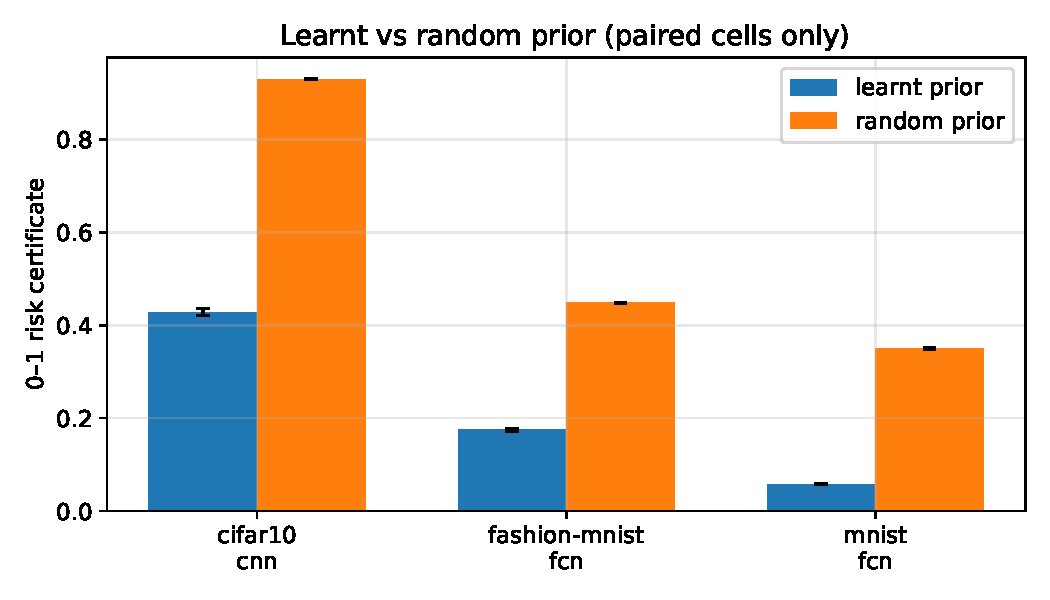
\includegraphics[width=0.7\linewidth]{fig_prior_comparison.pdf}
\caption{Learnt vs random prior certificate, shown only for cells where both
priors were run (including the CIFAR-10 control).}\label{fig:prior}
\end{figure}

The prior changes the KL a useful posterior must pay, and moves certificate
tightness a long way in every paired control (Figure~\ref{fig:prior}). On the
MNIST FCN $f_{\text{quad}}$ cell, going from a random to a learnt prior tightens
the certificate from $\CertMnistFcnFquadRand$ to $\CertMnistFcnFquadLearnt$ while
$\mathrm{KL}(Q\|P)$ falls from $\KlMnistFcnFquadRand$ to
$\KlMnistFcnFquadLearnt$ nats and the empirical Gibbs risk from
$\EmpMnistFcnFquadRand$ to $\EmpMnistFcnFquadLearnt$, so accuracy improves
alongside the certificate. The same direction holds on Fashion-MNIST
($\CertFashionmnistFcnFquadRand\!\to\!\CertFashionmnistFcnFquadLearnt$).

Which of the two terms does the work is a separate question, and the paired cells
answer it differently. The quantity to compare is not the raw KL but
$\mathrm{KL}/n_{\mathrm b}$, since $n_{\mathrm b}$ halves when the prior is
learnt. On MNIST the complexity term falls by $0.131$ against $0.087$ for the
empirical risk, so the complexity route is the larger. On Fashion-MNIST the two
are comparable and the ranking reverses: $0.082$ against $0.111$. On CIFAR-10 the
complexity term \emph{rises} by $0.033$, because the random-prior posterior barely
leaves its initialisation and so pays almost no KL, and the whole of the gain is
the empirical risk falling from $\EmpCifaronezeroCnnFquadRand$ to
$\EmpCifaronezeroCnnFquadLearnt$. The learnt prior tightens the certificate in
all three, then, but not by one mechanism: across these three paired cells the
dominant contribution shifts from the complexity term to the empirical risk. We
do not attribute that shift to difficulty, since architecture and budget change
along the same sequence.
The comparison is between two whole protocols rather than a pure prior-family
intervention: the random prior is independent of all of $S$ and so uses
$n_{\mathrm b}=|S|$, while the learnt prior uses the smaller
$n_{\mathrm b}=|S\setminus S_0|$ --- and still attains the tighter certificate
\emph{despite} that handicap. CIFAR-10 is the clearest case: a random prior
leaves the $f_{\text{quad}}$ certificate at $\CertCifaronezeroCnnFquadRand$,
whereas the learnt prior moves it to $\CertCifaronezeroCnnFquadLearnt$, formally
non-vacuous but still loose.

\paragraph{Architecture.} Where a CNN and an FCN are compared on the same dataset,
the convolutional model gives the tighter certificate: on MNIST the $f_{\text{quad}}$
learnt-prior certificate is $\CertMnistCnnFquadLearnt$ (CNN) versus
$\CertMnistFcnFquadLearnt$ (FCN), and on Fashion-MNIST
$\CertFashionmnistCnnFquadLearnt$ versus $\CertFashionmnistFcnFquadLearnt$.

\paragraph{Depth on CIFAR-10.} The reference obtains its tighter CIFAR-10
certificates with deeper networks than the nine-layer one used above, so we ran
its 13- and 15-layer architectures at the same five seeds and the same fixed
configuration. Within this $f_{\text{quad}}$ depth sweep the mean certificate
improves from nine to thirteen layers and worsens at fifteen:
$\CertCifaronezeroCnnFquadLearnt$, $\CertCifaronezeroCnnonethreeFquadLearnt$ and
$\CertCifaronezeroCnnonefiveFquadLearnt$ respectively. The 13-layer network also
improves the deployed error ($\PostmeanCifaronezeroCnnonethreeFquadLearnt$ versus
$\PostmeanCifaronezeroCnnFquadLearnt$), and the gain concentrates where the error
is: the per-class Gibbs risk of Section~\ref{sec:erroranalysis} falls from $0.448$
to $0.340$ on \emph{cat}, the hardest class. It is also the tightest CIFAR-10
certificate in the study, narrowly ahead of $f_{\text{classic}}$ at nine layers
($\CertCifaronezeroCnnFclassicLearnt$), and so the best of the three depths tested
under $f_{\text{quad}}$ and this configuration.

The 15-layer network does not continue the trend, for an instructive reason. Two
of its five seeds barely left the chance-level plateau, their prior networks
finishing at $0.866$ and $0.899$ error on the $S_0$ they were fitted to, against
a chance level of $0.900$: the second is chance to three decimals and the first
sits inside the criterion's five-point tolerance, both far from the at most
$0.228$ every other learnt prior reaches. The posterior is then initialised at an
essentially untrained prior, so the cell is not an instance of the protocol. Both are
registered as \texttt{not\_converged} and excluded by the criterion of
Section~\ref{sec:compute}; the remaining three give
$\CertCifaronezeroCnnonefiveFquadLearnt$, looser than the 13-layer result and far
more variable. That mean is conditional on convergence, so the failure rate is
part of the result: at fifteen layers this protocol trains $3$ of $5$ seeds,
against $5$ of $5$ everywhere else in the study. Twelve convolutional layers with
no normalisation, no warm-up and one fixed learning rate is past what it trains
reliably --- a limit of the fixed reduced-compute configuration rather than of the
method, and the price of holding one configuration across every cell.

\paragraph{Across datasets.} The learnt-prior $f_{\text{quad}}$ certificate rises
from MNIST ($\CertMnistFcnFquadLearnt$, FCN) through Fashion-MNIST
($\CertFashionmnistFcnFquadLearnt$, FCN) to CIFAR-10
($\CertCifaronezeroCnnFquadLearnt$, 9-layer CNN). The pattern is descriptive,
since architecture and compute budget change along it;
Section~\ref{sec:difficulty} is the controlled test of difficulty.

\subsection{Monte-Carlo sensitivity}\label{sec:mc}

\begin{figure}[h]\centering
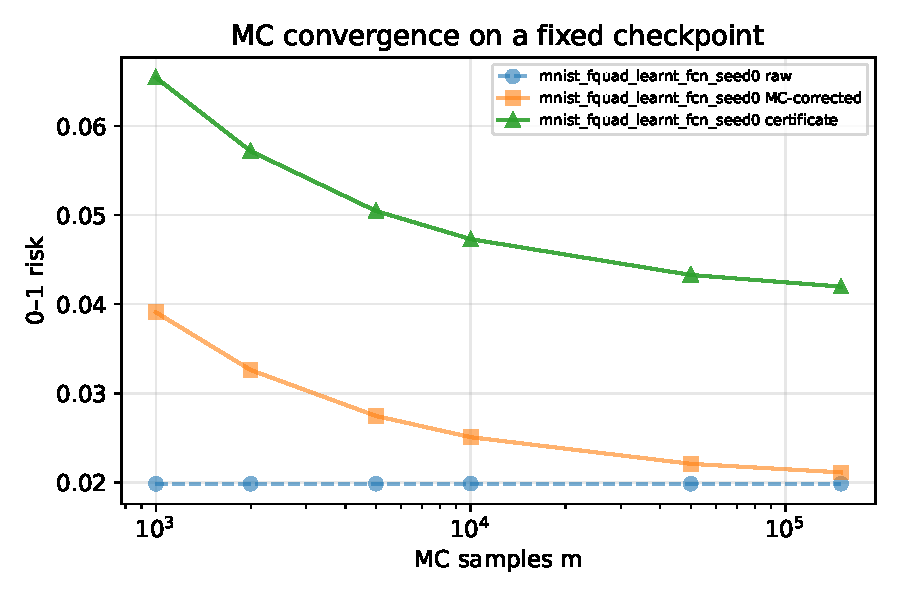
\includegraphics[width=0.7\linewidth]{fig_mc_convergence.pdf}
\caption{Final certificate versus the Monte-Carlo budget $m$ on a fixed checkpoint
with the Monte-Carlo estimate genuinely re-drawn at each budget, so both the
estimate and the finite-MC slack are free to move.}\label{fig:mc}
\end{figure}

The comparison above attributed our looser certificates partly to the Monte-Carlo
budget; this sweep measures that. Holding the posterior fixed at a saved
checkpoint and re-drawing at each budget, the certificate tightens monotonically
as $m$ grows and flattens well before the reference's budget
(Figure~\ref{fig:mc}). On the MNIST FCN $f_{\text{quad}}$ checkpoint it falls from
$0.0654$ at $m=1{,}000$ to $0.0572$ at our $m=2{,}000$ and $0.0420$ at the
reference's $m=150{,}000$ --- all the \emph{same} seed-0 checkpoint, which is why
the $m=2{,}000$ entry is not the five-seed mean $\CertMnistFcnFquadLearnt$ of
Table~\ref{tab:main}. Against the published $0.0279$, the re-draw recovers
$0.0152$ of this checkpoint's $0.0293$ gap. The rest is unexplained; the unmatched
grid search and epoch budget are plausible contributors we did not test
separately.

Two checks confirm that what moves is the slack and not the estimate. The raw
Monte-Carlo estimate is stable across the whole range ($0.01983$ at $m=1{,}000$
against $0.01984$ at $m=150{,}000$), as an unbiased estimator should be; and the
same curve computed analytically, holding that estimate fixed, agrees with the
measured one to within $2.2\times10^{-5}$ at every budget. Both curves are in the
artefact. A re-draw could have
moved the certificate either way; here it fell monotonically at every step, so
for this checkpoint and these draws the smaller $m$ was the conservative one.

\subsection{Small-data behaviour}\label{sec:smalldata}

\begin{table}[h]\centering\small
\caption{MNIST FCN $f_{\text{quad}}$/learnt versus training-data fraction, with the
corrected bound-set size $n_{\mathrm b}$ (mean~$\pm$~SD over seeds).}\label{tab:smalldata}
\begin{tabular}{r r r r r}
\toprule
\% data & $n_{\text{posterior}}$ & $n_{\text{bound}}$ & Emp.\ Gibbs & \textbf{Certificate} \\
\midrule
100\% & 60000 & 30000 & $0.0328\pm0.0006$ & $0.0580\pm0.0011$ \\
50\% & 30000 & 15000 & $0.0420\pm0.0024$ & $0.0777\pm0.0049$ \\
20\% & 12000 & 6000 & $0.0624\pm0.0034$ & $0.1196\pm0.0040$ \\
10\% & 6000 & 3000 & $0.0771\pm0.0035$ & $0.1520\pm0.0065$ \\
\bottomrule
\end{tabular}

\end{table}

\begin{figure}[h]\centering
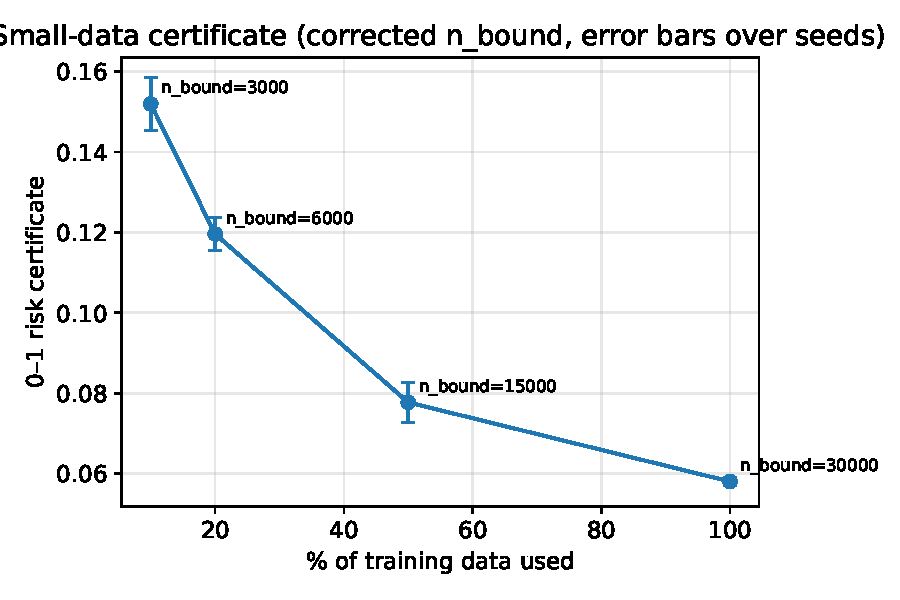
\includegraphics[width=0.7\linewidth]{fig_smalldata.pdf}
\caption{Certificate versus training-data fraction with the corrected
$n_{\mathrm b}$ and across-seed error bars.}\label{fig:smalldata}
\end{figure}

The certificate loosens monotonically as the training set shrinks
(Table~\ref{tab:smalldata} and Figure~\ref{fig:smalldata}): from
$\CertMnistFcnFquadLearnt$ at full data to
$\CertMnistFcnFquadLearntPtFiveZero$ ($50\%$),
$\CertMnistFcnFquadLearntPtTwoZero$ ($20\%$) and
$\CertMnistFcnFquadLearntPtOneZero$ at $10\%$ of the data
($n_{\mathrm b}=3{,}000$). The certificate increases monotonically as the data
fraction falls, and each step exceeds the across-seed spread at that setting. The small-data runs show most directly why the
sample-count audit matters. The certificate denominator is the bound-set size
$n_{\mathrm b}$, which at $10\%$ data is $3{,}000$, whereas taking it to be the
size of the full training set would instead give $60{,}000$. Using the full
dataset size understates the complexity term and reports a spuriously tight
certificate at small $n$: on these same five checkpoints the wrong denominator
returns $0.092$ where the correct one returns
$\CertMnistFcnFquadLearntPtOneZero$, hiding most of the degradation. The bound
stays non-vacuous down to $10\%$ of the data, so the degradation is graceful, but
it is far from the near-flat behaviour a mis-counted $n$ would suggest.

\subsection{Controlled difficulty}\label{sec:difficulty}

\begin{figure}[h]\centering
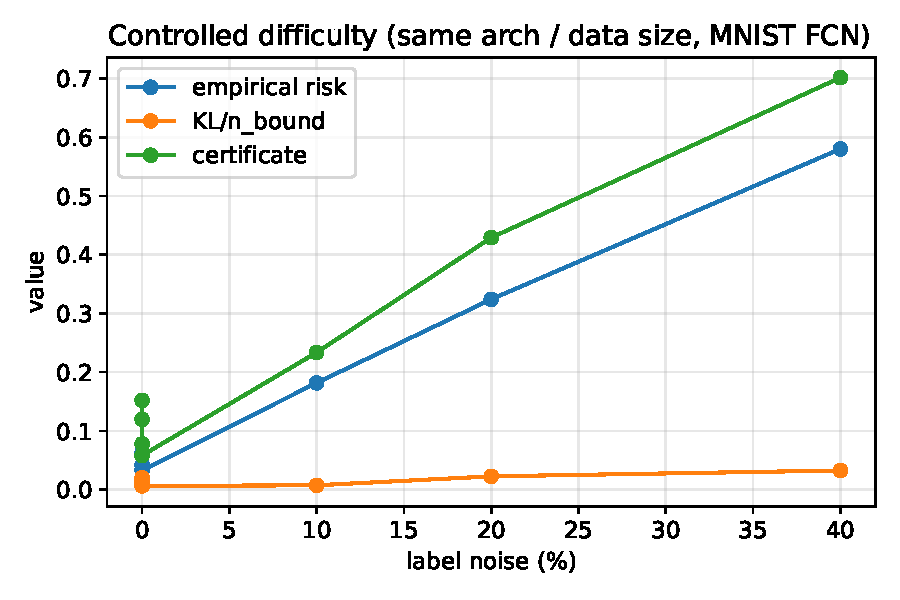
\includegraphics[width=0.7\linewidth]{fig_difficulty.pdf}
\caption{Empirical risk, $\mathrm{KL}/n_{\mathrm b}$ and certificate versus
label-noise level for the MNIST FCN $f_{\text{quad}}$/learnt cell (architecture,
sample size and compute held fixed).}\label{fig:difficulty}
\end{figure}

The cross-dataset trend above could not separate difficulty from the architecture
and budget that change alongside it; this study removes that confound. With
architecture, sample size and compute held fixed and label noise injected into the
MNIST FCN $f_{\text{quad}}$ learnt-prior cell, the certificate rises monotonically
with the noise level (Figure~\ref{fig:difficulty}), from
$\CertMnistFcnFquadLearnt$ at no noise to
$\CertMnistFcnFquadLearntLnOneZero$, $\CertMnistFcnFquadLearntLnTwoZero$ and
$\CertMnistFcnFquadLearntLnFourZero$ at $10$, $20$ and $40\%$ noise. Successive
noise levels are separated by far more than the across-seed spread
(Figure~\ref{fig:difficulty}). The increase is
driven mainly by the empirical-risk term, since corrupted labels raise the error
floor that any posterior must pay on $S_{\mathrm b}$, with a smaller rise in
$\mathrm{KL}/n_{\mathrm b}$. Because
every other factor is held fixed, this is the one place we attribute a difficulty
effect to the intervention itself. The certified quantity here is the Gibbs risk
on the \emph{noisy-label} distribution the model is trained and evaluated
against, not on clean labels.

\subsection{The certified predictor versus the deployed one}\label{sec:deploygap}

Table~\ref{tab:main} also lets us compare the predictor the certificate covers
against the one a user would deploy. The posterior-mean test error is below the
stochastic (Gibbs) error in every learnt-prior cell, though not universally: on
the CIFAR-10 data-free-prior cell, where neither predictor has learnt much, the
ordering reverses. The finite ensemble is usually below the stochastic error but
is not uniformly below the posterior mean. On the MNIST FCN $f_{\text{quad}}$
cell the stochastic error is $\StochMnistFcnFquadLearnt$ against a posterior mean
of $\PostmeanMnistFcnFquadLearnt$, and the same direction holds on Fashion-MNIST
and CIFAR-10 with a learnt prior. The gap is consistent across the learnt-prior
cells and not negligible, at roughly a fifth of the stochastic error on the MNIST
cell, and by Section~\ref{sec:scope} it does not transfer the certificate to the
posterior mean, so a user needing a guarantee for the deterministic network does
not have one here. Closing that gap is the clearest theoretical extension of the
project.

\subsection{Where the error falls}\label{sec:erroranalysis}

The certificate bounds an aggregate risk, and it is informative to see how the
error distributes across classes, since that is what the empirical-risk term
integrates over. Figure~\ref{fig:confusion} shows the posterior-mean confusion
matrices on the two harder datasets. On Fashion-MNIST the error concentrates in
the upper-body garments, the worst class being \emph{shirt}, confused mainly with
\emph{pullover}, \emph{coat} and \emph{T-shirt}, while the footwear classes are
almost perfectly separated; on CIFAR-10 it sits in \emph{cat}, \emph{dog} and
\emph{bird}, with the rigid vehicle classes much easier. Those matrices describe
the posterior-mean predictor on the test
set, which is not the object the certificate bounds, so we also decomposed the
certified quantity itself: the Monte-Carlo Gibbs risk on $S_{\mathrm b}$,
accumulated by true class over the same $m=2{,}000$ draws that produce the
certificate, on the seed-$0$ checkpoint of each cell. What is decomposed is the
Monte-Carlo average $\bar{R}$, before the finite-sample correction
of~\eqref{eq:mc}, so the per-class values below sit on that scale rather than on
the scale of the corrected $\overline{R}^{+}$ quoted elsewhere. Its class average reproduces the
run's own aggregate estimate to within $10^{-4}$, which is the check that the
decomposition is of the right quantity.

The certified risk concentrates in the same places, and more sharply: on
Fashion-MNIST the Gibbs risk on \emph{shirt} is $0.293$ against a dataset-wide
$0.108$ on the same scale, and on CIFAR-10 it is \emph{cat} $0.448$,
\emph{dog} $0.383$ and \emph{bird} $0.366$ against $0.264$ for the nine-layer
network. The worst class carries close to three times the average risk the bound
integrates over on Fashion-MNIST and about $1.7$ times it on CIFAR-10. That is
what the empirical-risk term of Section~\ref{sec:main} is made of, and why a
well-controlled KL cannot pull the harder datasets into the MNIST range. It also
marks a boundary of the method: the certificate is one number over all classes, so
a deployment that cares about the worst class is not served by it.

\begin{figure}[h]\centering
\begin{subfigure}{0.49\linewidth}\centering
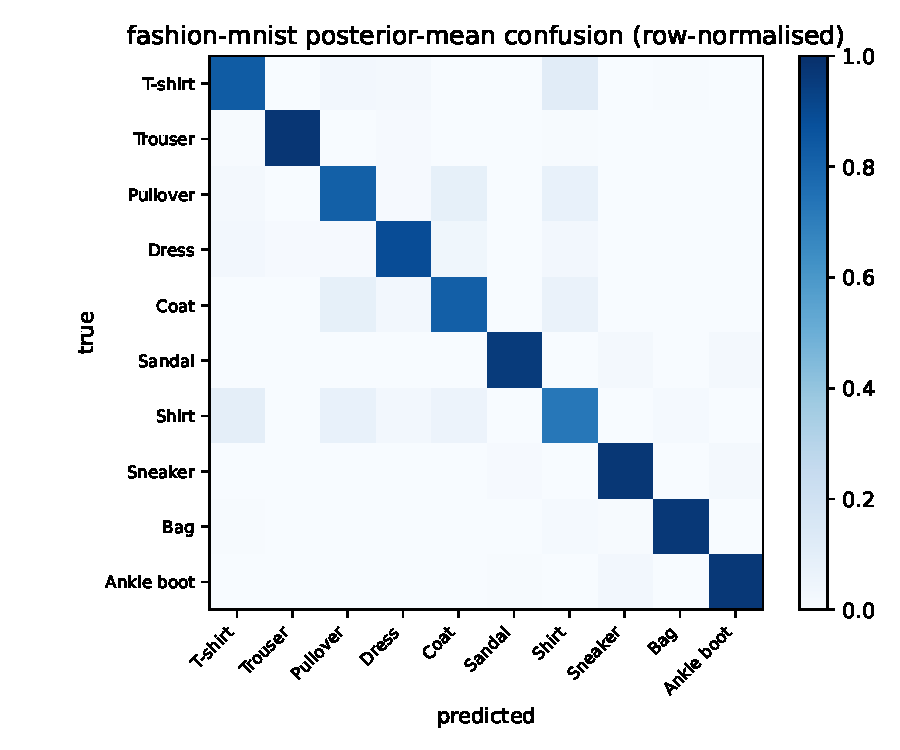
\includegraphics[width=\linewidth]{fig_confusion_fashion-mnist.pdf}
\caption{Fashion-MNIST}\end{subfigure}
\begin{subfigure}{0.49\linewidth}\centering
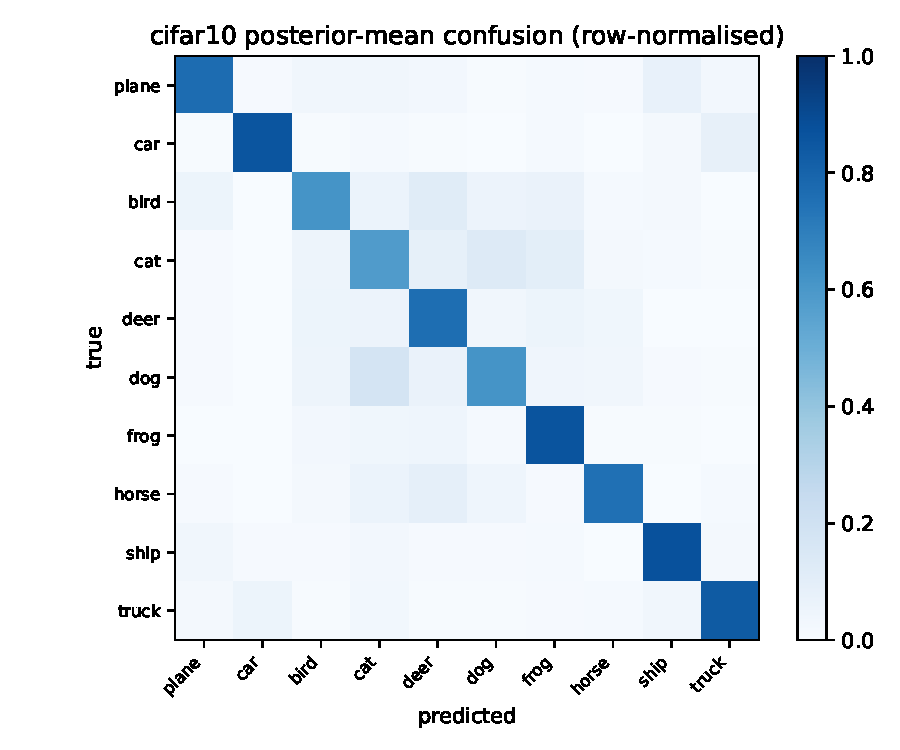
\includegraphics[width=\linewidth]{fig_confusion_cifar10.pdf}
\caption{CIFAR-10}\end{subfigure}
\caption{Posterior-mean confusion matrices (row-normalised) on the two harder
datasets. The error concentrates in visually similar classes, which raises the
empirical Gibbs risk that the certificate is built on.}\label{fig:confusion}
\end{figure}

\section{Evaluation and Reflection}\label{sec:evaluation}

\subsection{Evaluation strategy}\label{sec:evalstrategy}

The evaluation is organised around the questions of the introduction rather than
a single accuracy number, because the object of study is the certificate and its
trustworthiness. Correctness is checked before any result is interpreted: each
audited condition has a unit test, and every certificate is recomputed from its
saved ingredients. Every cell runs five seeds and is reported as a mean with a
standard deviation, the sole exception being the CIFAR-10 15-layer cell, where
two runs did not train. The two claims easiest to confound, the effect of the
prior and of difficulty, rest on controlled comparisons instead: a paired
learnt-versus-random prior on every dataset, and a label-noise sweep with
architecture and sample size held fixed. Causal claims are restricted to those.

\subsection{Threats to validity}\label{sec:threats}

The main threats concern differences from the reference protocol and limits on
how the results can be interpreted. On the first, the reduced-compute protocol of
Section~\ref{sec:protocol} deviates in several ways and only one of them, the
Monte-Carlo budget, has been measured (Section~\ref{sec:mc}); the absent
hyper-parameter search and the epoch budget can move the certificate either way
and we do not bound them. One threat is internal to our own correction: the union
over prior scales needs a candidate set fixed independently of the bound set, and
ours was written down afterwards (Section~\ref{sec:confidence}). The exposure is
small, since the grid covers every scale the probe could plausibly have returned,
but that is an assumption about our procedure, not something the data confirms.

The interpretive limits concern the certified predictor, the cross-dataset
comparison, the prior comparison and seed variability. Only the Gibbs classifier
is certified (Section~\ref{sec:scope}); a formal bound for the deterministic
predictors via the C-bound is left to future work. As noted in
Section~\ref{sec:main}, the cross-dataset comparison is descriptive because its
confounders are not controlled, and the label-noise study is where a difficulty
claim is made instead. Even the prior comparison, our most controlled effect, compares
two whole protocols rather than one isolated factor, which is why a CIFAR-10
random-prior control is included rather than inferred from the easier datasets.
Finally, the across-seed spread is the variability of the training procedure and
must not be read as a confidence interval on the certificate: the PAC-Bayes
guarantee is about one trained model, holding with probability at least
$1-\delta_{\mathrm{MC}}-\delta_{\mathrm{PAC}}=0.99$.

\subsection{Limitations}\label{sec:limitations}

A non-vacuous certificate is not necessarily a useful one: a CIFAR-10
certificate below $1$ may still be too loose to drive a deployment decision.
Depth is varied only in the CIFAR-10 $f_{\text{quad}}$ sweep and never with
width; we test no modality beyond image benchmarks, and implement neither the
differentially-private-prior nor the majority-vote route. The audit corrects and
tests the pipeline issues we identified, but is not an exhaustive verification of
the upstream code.

\subsection{Reflection on the project process}\label{sec:reflection}

The most useful lesson from the project was how easily a reproduction of a
certificate can be wrong in a way that nothing flags. The original difficulty
ladder appeared to hold, the small-data certificate appeared to stay tight, and
the objective ordering appeared to match the literature, until each was traced
back to a specific step in the pipeline. The sample-count convention is the
clearest example: at $10\%$ data, putting the full $60{,}000$ in the denominator
instead of the true $n_{\mathrm b}=3{,}000$ makes a certificate that is really
$0.152$ read as $0.092$, and either figure looks plausible. That
experience shifted the project towards verifiable certificates, and motivated
building the unit tests and the registry before the headline runs.

With hindsight, one thing would have been done much earlier: profiling. The data
pipeline, not the network, dominated wall-clock time, and the Monte-Carlo
evaluation ran in far smaller batches than the hardware needed. Fixing both left
the reported numbers untouched, since neither changes what is computed, but it
turned the full matrix from a budget question into a routine one. The registry,
the per-run provenance and the regeneration of every results figure from raw results are
what make these certificates independently checkable, and on this evidence they
belong in the result rather than after it.

\section{Conclusion}\label{sec:conclusion}

This dissertation partially reproduced selected PAC-Bayes-with-Backprop cells on
MNIST under a reduced-compute protocol, extended them to Fashion-MNIST and
CIFAR-10, and re-implemented the certificate-computation pipeline with corrected
bookkeeping.

On reproduction, the corrected pipeline matches the reference's MNIST stochastic
test errors to within $\ReproStochDeltaAbsMax$ on all four target cells, with
the sign of the difference varying between them. The certificates are uniformly
looser; the Monte-Carlo sweep accounts for roughly half of the gap on the cell
examined in detail, and the rest coincides with protocol differences, chiefly the
absent per-cell grid search, that we identified but did not measure. The
reproduction is therefore complete on the predictive metrics and partial on the
certificate. Decomposing it revealed effects that test error alone does not: it
separates into the empirical Gibbs risk and a complexity term scaling with
$\mathrm{KL}/n_{\mathrm b}$, and a learnt prior tightens it in every paired
comparison we ran, though not by the same route each time. Measured
on the scale that enters the bound, $\mathrm{KL}/n_{\mathrm b}$, the complexity
term is the larger route only on MNIST; on Fashion-MNIST the two routes are
comparable, and on CIFAR-10 the learnt prior pays \emph{more} complexity and wins
entirely on empirical risk. That decomposition is what makes the certificate
sensitive in the ways the sensitivity analysis probes --- to the prior, the
bound-set size, the Monte-Carlo budget and the seed --- and it is where the audit
proves its worth, since correcting the bound-set sample count alone loosens the
small-data certificates substantially. Difficulty was
therefore tested in the one design that controls for it: with everything but the
label noise held constant, the noise raises the empirical-risk term and, through
the PAC-Bayes-kl inversion, the certificate, so the effect can be attributed to
the perturbation itself, with the proviso that the certified quantity is then the
Gibbs risk on the noisy-label distribution.

Together these results show that PAC-Bayes-with-Backprop delivered formally
non-vacuous certificates in all $23$ reported cells, none reaching $1$ --- a
statement about runs that trained, since the $15$-layer cell is the mean of its
three converged seeds. Non-vacuous and useful are different thresholds, though:
the loosest, CIFAR-10 under $f_{\text{bbb}}$, is
$\CertCifaronezeroCnnBbbLearnt$, certifying almost nothing a practitioner would
act on, and tight certificates arrived only on the easier benchmarks. In all
three paired $f_{\text{quad}}$ controls the data-dependent prior produced a large
tightening --- not the largest effect in the study, since $40\%$ label noise
moves the same MNIST certificate about twice as far.
The value of any such number depends on the implementation that produced it, and
several conventions in the reference required correction in our
re-implementation. The main contribution of the project is that corrected, tested
pipeline: reliable certificates require correct sample counts, confidence
accounting, Monte-Carlo aggregation and seed handling, together with enough
provenance to re-derive each reported value.

The clearest direction for further work is to close the gap
between the certified Gibbs classifier and the deterministic predictor actually
deployed. The C-bound of \textcite{lacasse2006,germain2015} relates the
majority-vote risk to the mean and variance of the Gibbs risk, and adapting it to
the objectives used here would give a formal guarantee for a deterministic
predictor. Which one matters: the C-bound governs the majority vote induced by
$Q$, the limit of the ensemble predictor, not the posterior-mean network whose
error we report, so a guarantee for the latter would remain open. On
the empirical side, the full-budget re-draw reported here removes one identified
source of the discrepancy but not the absent grid search, which is what a
reference-matched hyper-parameter search would settle.
The CIFAR-10 results invite two extensions: the deeper 13- and 15-layer
architectures that the reference shows give tighter bounds, and the
differentially-private prior route, which would let the prior use all of the data
and is the more promising way to attack the high empirical risk that, as the
error analysis shows, is what keeps CIFAR-10 certificates loose. Finally, the
controlled-difficulty design could be broadened from label noise to input
corruption and class overlap, to test whether the empirical-risk mechanism
identified here is the dominant one across different notions of difficulty.



%%%%%%%%%%%%%%%%%% REFERENCES %%%%%%%%%%%%%%%%%%
%\clearpage % uncomment to start on a new page if wanted
\printbibliography[title={References},heading=bibintoc] % a single list of references for the whole thesis



%%%%%%%%%%%%%%%%%% APPENDICES %%%%%%%%%%%%%%%%%%
\begin{uomappendix}
    \section{Per-seed complete results}\label{app:perseed}
    Table~\ref{tab:perseed} gives per-seed results for all $113$ reported runs,
generated from the results registry. Each row is one run, whose configuration,
data split, checkpoints and metrics are retained and whose inclusion or exclusion
is recorded in the registry. The registry holds $115$ runs; the two that do not
appear here are the learnt-prior runs whose prior network never left the
chance-level plateau, at $0.866$ and $0.899$ error on $S_0$, excluded under the
criterion stated in Section~\ref{sec:compute}.

The \textbf{Condition} column identifies which study a row belongs to.
\emph{Headline} rows use the full training set with clean labels and are the cells
of Table~\ref{tab:main}, run at five seeds ($0$--$4$). \emph{Data~$p\%$} rows are
the small-data sweep of Section~\ref{sec:smalldata}, retrained on a uniformly
random $p\%$ of the training set drawn without reading any label, at five seeds
($0$--$4$).
\emph{Noise~$\eta\%$} rows are the controlled-difficulty study of
Section~\ref{sec:difficulty}, with a fraction $\eta$ of the labels of $S$
corrupted to a uniformly random different class, also at five seeds. Rows sharing
a dataset, model, prior, objective and condition differ only in their seed.

Column $n_{\mathrm b}$ is the bound-set size actually used in the certificate, so
it varies with both the prior family and the training-data fraction. The risk
certificate is the $0$--$1$ PAC-Bayes-kl bound on the Gibbs risk at confidence
$0.99$, per certificate and per run. ``Stoch~/ PM~/ Ens'' are the stochastic,
posterior-mean and ensemble test errors, which are descriptive deployment metrics
and carry no guarantee; for the noise rows they are measured against clean test
labels, whereas the certificate in the same row refers to the corrupted-label
distribution, so the two are not comparable within those rows.

{\scriptsize\begin{longtable}[]{@{}lllllr r r r r r@{}}
\caption{Per-seed results for all 113 reported runs, one row per run.}\label{tab:perseed}\\
\toprule\noalign{}
Dataset & Model & Prior & Obj. & Condition & Seed & $n_{\text{b}}$ & Cert & Stoch & PM & Ens \\
\midrule\noalign{}\endfirsthead
\multicolumn{11}{@{}l}{\emph{Table \thetable\ continued from previous page}}\\
\toprule\noalign{}
Dataset & Model & Prior & Obj. & Condition & Seed & $n_{\text{b}}$ & Cert & Stoch & PM & Ens \\
\midrule\noalign{}\endhead
\midrule\multicolumn{11}{r@{}}{\emph{continued on next page}}\\\endfoot
\bottomrule\noalign{}\endlastfoot
CIFAR-10 & CNN & learnt & $f_{\text{bbb}}$ & headline & 0 & 25000 & 0.9796 & 0.2445 & 0.2181 & 0.2055 \\
CIFAR-10 & CNN & learnt & $f_{\text{bbb}}$ & headline & 1 & 25000 & 0.9817 & 0.2400 & 0.2163 & 0.2030 \\
CIFAR-10 & CNN & learnt & $f_{\text{bbb}}$ & headline & 2 & 25000 & 0.9804 & 0.2382 & 0.2181 & 0.2029 \\
CIFAR-10 & CNN & learnt & $f_{\text{bbb}}$ & headline & 3 & 25000 & 0.9824 & 0.2557 & 0.2214 & 0.2094 \\
CIFAR-10 & CNN & learnt & $f_{\text{bbb}}$ & headline & 4 & 25000 & 0.9762 & 0.2274 & 0.2072 & 0.1947 \\
\addlinespace[2pt]
CIFAR-10 & CNN & learnt & $f_{\text{classic}}$ & headline & 0 & 25000 & 0.3894 & 0.2865 & 0.2610 & 0.2391 \\
CIFAR-10 & CNN & learnt & $f_{\text{classic}}$ & headline & 1 & 25000 & 0.3996 & 0.2940 & 0.2692 & 0.2510 \\
CIFAR-10 & CNN & learnt & $f_{\text{classic}}$ & headline & 2 & 25000 & 0.3950 & 0.2918 & 0.2558 & 0.2408 \\
CIFAR-10 & CNN & learnt & $f_{\text{classic}}$ & headline & 3 & 25000 & 0.4015 & 0.3014 & 0.2691 & 0.2528 \\
CIFAR-10 & CNN & learnt & $f_{\text{classic}}$ & headline & 4 & 25000 & 0.3808 & 0.2771 & 0.2523 & 0.2355 \\
\addlinespace[2pt]
CIFAR-10 & CNN & learnt & $f_{\text{quad}}$ & headline & 0 & 25000 & 0.4244 & 0.2788 & 0.2564 & 0.2314 \\
CIFAR-10 & CNN & learnt & $f_{\text{quad}}$ & headline & 1 & 25000 & 0.4336 & 0.2819 & 0.2581 & 0.2403 \\
CIFAR-10 & CNN & learnt & $f_{\text{quad}}$ & headline & 2 & 25000 & 0.4282 & 0.2826 & 0.2460 & 0.2306 \\
CIFAR-10 & CNN & learnt & $f_{\text{quad}}$ & headline & 3 & 25000 & 0.4351 & 0.2907 & 0.2596 & 0.2430 \\
CIFAR-10 & CNN & learnt & $f_{\text{quad}}$ & headline & 4 & 25000 & 0.4170 & 0.2671 & 0.2425 & 0.2258 \\
\addlinespace[2pt]
CIFAR-10 & CNN & data-free & $f_{\text{quad}}$ & headline & 0 & 50000 & 0.9291 & 0.8957 & 0.9000 & 0.8942 \\
CIFAR-10 & CNN & data-free & $f_{\text{quad}}$ & headline & 1 & 50000 & 0.9302 & 0.9006 & 0.9000 & 0.8966 \\
CIFAR-10 & CNN & data-free & $f_{\text{quad}}$ & headline & 2 & 50000 & 0.9295 & 0.8960 & 0.9000 & 0.8994 \\
CIFAR-10 & CNN & data-free & $f_{\text{quad}}$ & headline & 3 & 50000 & 0.9294 & 0.8989 & 0.9000 & 0.9033 \\
CIFAR-10 & CNN & data-free & $f_{\text{quad}}$ & headline & 4 & 50000 & 0.9304 & 0.8977 & 0.9000 & 0.8984 \\
\addlinespace[2pt]
CIFAR-10 & cnn13 & learnt & $f_{\text{quad}}$ & headline & 0 & 25000 & 0.3849 & 0.2174 & 0.1794 & 0.1717 \\
CIFAR-10 & cnn13 & learnt & $f_{\text{quad}}$ & headline & 1 & 25000 & 0.3934 & 0.2247 & 0.1817 & 0.1718 \\
CIFAR-10 & cnn13 & learnt & $f_{\text{quad}}$ & headline & 2 & 25000 & 0.3849 & 0.2160 & 0.1757 & 0.1700 \\
CIFAR-10 & cnn13 & learnt & $f_{\text{quad}}$ & headline & 3 & 25000 & 0.3864 & 0.2154 & 0.1770 & 0.1682 \\
CIFAR-10 & cnn13 & learnt & $f_{\text{quad}}$ & headline & 4 & 25000 & 0.3908 & 0.2273 & 0.1818 & 0.1747 \\
\addlinespace[2pt]
CIFAR-10 & cnn15 & learnt & $f_{\text{quad}}$ & headline & 1 & 25000 & 0.5284 & 0.3380 & 0.2795 & 0.2753 \\
CIFAR-10 & cnn15 & learnt & $f_{\text{quad}}$ & headline & 2 & 25000 & 0.4425 & 0.2604 & 0.2025 & 0.2037 \\
CIFAR-10 & cnn15 & learnt & $f_{\text{quad}}$ & headline & 3 & 25000 & 0.4456 & 0.2556 & 0.1976 & 0.1955 \\
\addlinespace[2pt]
Fashion-MNIST & CNN & learnt & $f_{\text{quad}}$ & headline & 0 & 30000 & 0.1658 & 0.0924 & 0.0864 & 0.0847 \\
Fashion-MNIST & CNN & learnt & $f_{\text{quad}}$ & headline & 1 & 30000 & 0.1739 & 0.0932 & 0.0870 & 0.0838 \\
Fashion-MNIST & CNN & learnt & $f_{\text{quad}}$ & headline & 2 & 30000 & 0.1627 & 0.0908 & 0.0850 & 0.0805 \\
Fashion-MNIST & CNN & learnt & $f_{\text{quad}}$ & headline & 3 & 30000 & 0.1638 & 0.0971 & 0.0881 & 0.0837 \\
Fashion-MNIST & CNN & learnt & $f_{\text{quad}}$ & headline & 4 & 30000 & 0.1708 & 0.0920 & 0.0867 & 0.0832 \\
\addlinespace[2pt]
Fashion-MNIST & FCN & learnt & $f_{\text{bbb}}$ & headline & 0 & 30000 & 0.6616 & 0.1111 & 0.1025 & 0.1001 \\
Fashion-MNIST & FCN & learnt & $f_{\text{bbb}}$ & headline & 1 & 30000 & 0.6656 & 0.1097 & 0.1000 & 0.0996 \\
Fashion-MNIST & FCN & learnt & $f_{\text{bbb}}$ & headline & 2 & 30000 & 0.6573 & 0.1125 & 0.1018 & 0.0993 \\
Fashion-MNIST & FCN & learnt & $f_{\text{bbb}}$ & headline & 3 & 30000 & 0.6692 & 0.1139 & 0.1042 & 0.0997 \\
Fashion-MNIST & FCN & learnt & $f_{\text{bbb}}$ & headline & 4 & 30000 & 0.6622 & 0.1119 & 0.1005 & 0.0978 \\
\addlinespace[2pt]
Fashion-MNIST & FCN & learnt & $f_{\text{classic}}$ & headline & 0 & 30000 & 0.1574 & 0.1228 & 0.1148 & 0.1122 \\
Fashion-MNIST & FCN & learnt & $f_{\text{classic}}$ & headline & 1 & 30000 & 0.1593 & 0.1178 & 0.1125 & 0.1084 \\
Fashion-MNIST & FCN & learnt & $f_{\text{classic}}$ & headline & 2 & 30000 & 0.1556 & 0.1224 & 0.1166 & 0.1139 \\
Fashion-MNIST & FCN & learnt & $f_{\text{classic}}$ & headline & 3 & 30000 & 0.1586 & 0.1219 & 0.1137 & 0.1110 \\
Fashion-MNIST & FCN & learnt & $f_{\text{classic}}$ & headline & 4 & 30000 & 0.1600 & 0.1170 & 0.1103 & 0.1065 \\
\addlinespace[2pt]
Fashion-MNIST & FCN & learnt & $f_{\text{quad}}$ & headline & 0 & 30000 & 0.1740 & 0.1208 & 0.1130 & 0.1110 \\
Fashion-MNIST & FCN & learnt & $f_{\text{quad}}$ & headline & 1 & 30000 & 0.1763 & 0.1162 & 0.1089 & 0.1061 \\
Fashion-MNIST & FCN & learnt & $f_{\text{quad}}$ & headline & 2 & 30000 & 0.1713 & 0.1207 & 0.1143 & 0.1092 \\
Fashion-MNIST & FCN & learnt & $f_{\text{quad}}$ & headline & 3 & 30000 & 0.1741 & 0.1209 & 0.1124 & 0.1088 \\
Fashion-MNIST & FCN & learnt & $f_{\text{quad}}$ & headline & 4 & 30000 & 0.1776 & 0.1145 & 0.1057 & 0.1040 \\
\addlinespace[2pt]
Fashion-MNIST & FCN & data-free & $f_{\text{quad}}$ & headline & 0 & 60000 & 0.4487 & 0.2219 & 0.1979 & 0.1828 \\
Fashion-MNIST & FCN & data-free & $f_{\text{quad}}$ & headline & 1 & 60000 & 0.4463 & 0.2184 & 0.1890 & 0.1800 \\
Fashion-MNIST & FCN & data-free & $f_{\text{quad}}$ & headline & 2 & 60000 & 0.4489 & 0.2231 & 0.1898 & 0.1803 \\
Fashion-MNIST & FCN & data-free & $f_{\text{quad}}$ & headline & 3 & 60000 & 0.4478 & 0.2334 & 0.1851 & 0.1824 \\
Fashion-MNIST & FCN & data-free & $f_{\text{quad}}$ & headline & 4 & 60000 & 0.4485 & 0.2303 & 0.1836 & 0.1813 \\
\addlinespace[2pt]
MNIST & CNN & learnt & $f_{\text{quad}}$ & headline & 0 & 30000 & 0.0373 & 0.0095 & 0.0082 & 0.0083 \\
MNIST & CNN & learnt & $f_{\text{quad}}$ & headline & 1 & 30000 & 0.0369 & 0.0107 & 0.0103 & 0.0100 \\
MNIST & CNN & learnt & $f_{\text{quad}}$ & headline & 2 & 30000 & 0.0364 & 0.0124 & 0.0103 & 0.0105 \\
MNIST & CNN & learnt & $f_{\text{quad}}$ & headline & 3 & 30000 & 0.0389 & 0.0110 & 0.0096 & 0.0102 \\
MNIST & CNN & learnt & $f_{\text{quad}}$ & headline & 4 & 30000 & 0.0352 & 0.0104 & 0.0092 & 0.0087 \\
\addlinespace[2pt]
MNIST & FCN & learnt & $f_{\text{bbb}}$ & headline & 0 & 30000 & 0.2657 & 0.0191 & 0.0151 & 0.0154 \\
MNIST & FCN & learnt & $f_{\text{bbb}}$ & headline & 1 & 30000 & 0.2631 & 0.0175 & 0.0149 & 0.0148 \\
MNIST & FCN & learnt & $f_{\text{bbb}}$ & headline & 2 & 30000 & 0.2585 & 0.0186 & 0.0141 & 0.0140 \\
MNIST & FCN & learnt & $f_{\text{bbb}}$ & headline & 3 & 30000 & 0.2762 & 0.0191 & 0.0147 & 0.0145 \\
MNIST & FCN & learnt & $f_{\text{bbb}}$ & headline & 4 & 30000 & 0.2653 & 0.0192 & 0.0156 & 0.0155 \\
\addlinespace[2pt]
MNIST & FCN & learnt & $f_{\text{classic}}$ & headline & 0 & 30000 & 0.0450 & 0.0247 & 0.0206 & 0.0204 \\
MNIST & FCN & learnt & $f_{\text{classic}}$ & headline & 1 & 30000 & 0.0448 & 0.0237 & 0.0185 & 0.0193 \\
MNIST & FCN & learnt & $f_{\text{classic}}$ & headline & 2 & 30000 & 0.0450 & 0.0230 & 0.0197 & 0.0194 \\
MNIST & FCN & learnt & $f_{\text{classic}}$ & headline & 3 & 30000 & 0.0465 & 0.0235 & 0.0191 & 0.0191 \\
MNIST & FCN & learnt & $f_{\text{classic}}$ & headline & 4 & 30000 & 0.0461 & 0.0253 & 0.0182 & 0.0189 \\
\addlinespace[2pt]
MNIST & FCN & learnt & $f_{\lambda}$ & headline & 0 & 30000 & 0.0766 & 0.0214 & 0.0162 & 0.0169 \\
MNIST & FCN & learnt & $f_{\lambda}$ & headline & 1 & 30000 & 0.0767 & 0.0209 & 0.0173 & 0.0172 \\
MNIST & FCN & learnt & $f_{\lambda}$ & headline & 2 & 30000 & 0.0768 & 0.0206 & 0.0171 & 0.0163 \\
MNIST & FCN & learnt & $f_{\lambda}$ & headline & 3 & 30000 & 0.0795 & 0.0211 & 0.0167 & 0.0171 \\
MNIST & FCN & learnt & $f_{\lambda}$ & headline & 4 & 30000 & 0.0785 & 0.0214 & 0.0176 & 0.0163 \\
\addlinespace[2pt]
MNIST & FCN & learnt & $f_{\text{quad}}$ & data 10\% & 0 & 3000 & 0.1487 & 0.0623 & 0.0544 & 0.0537 \\
MNIST & FCN & learnt & $f_{\text{quad}}$ & data 10\% & 1 & 3000 & 0.1628 & 0.0630 & 0.0537 & 0.0544 \\
MNIST & FCN & learnt & $f_{\text{quad}}$ & data 10\% & 2 & 3000 & 0.1488 & 0.0628 & 0.0562 & 0.0570 \\
MNIST & FCN & learnt & $f_{\text{quad}}$ & data 10\% & 3 & 3000 & 0.1532 & 0.0631 & 0.0541 & 0.0566 \\
MNIST & FCN & learnt & $f_{\text{quad}}$ & data 10\% & 4 & 3000 & 0.1463 & 0.0648 & 0.0571 & 0.0583 \\
\addlinespace[2pt]
MNIST & FCN & learnt & $f_{\text{quad}}$ & data 20\% & 0 & 6000 & 0.1268 & 0.0452 & 0.0365 & 0.0397 \\
MNIST & FCN & learnt & $f_{\text{quad}}$ & data 20\% & 1 & 6000 & 0.1178 & 0.0482 & 0.0383 & 0.0392 \\
MNIST & FCN & learnt & $f_{\text{quad}}$ & data 20\% & 2 & 6000 & 0.1183 & 0.0480 & 0.0407 & 0.0414 \\
MNIST & FCN & learnt & $f_{\text{quad}}$ & data 20\% & 3 & 6000 & 0.1172 & 0.0466 & 0.0391 & 0.0397 \\
MNIST & FCN & learnt & $f_{\text{quad}}$ & data 20\% & 4 & 6000 & 0.1178 & 0.0459 & 0.0395 & 0.0401 \\
\addlinespace[2pt]
MNIST & FCN & learnt & $f_{\text{quad}}$ & data 50\% & 0 & 15000 & 0.0699 & 0.0297 & 0.0239 & 0.0250 \\
MNIST & FCN & learnt & $f_{\text{quad}}$ & data 50\% & 1 & 15000 & 0.0830 & 0.0315 & 0.0244 & 0.0252 \\
MNIST & FCN & learnt & $f_{\text{quad}}$ & data 50\% & 2 & 15000 & 0.0777 & 0.0280 & 0.0218 & 0.0233 \\
MNIST & FCN & learnt & $f_{\text{quad}}$ & data 50\% & 3 & 15000 & 0.0773 & 0.0321 & 0.0247 & 0.0259 \\
MNIST & FCN & learnt & $f_{\text{quad}}$ & data 50\% & 4 & 15000 & 0.0808 & 0.0305 & 0.0230 & 0.0246 \\
\addlinespace[2pt]
MNIST & FCN & learnt & $f_{\text{quad}}$ & headline & 0 & 30000 & 0.0572 & 0.0216 & 0.0170 & 0.0191 \\
MNIST & FCN & learnt & $f_{\text{quad}}$ & headline & 1 & 30000 & 0.0574 & 0.0216 & 0.0178 & 0.0177 \\
MNIST & FCN & learnt & $f_{\text{quad}}$ & headline & 2 & 30000 & 0.0572 & 0.0216 & 0.0178 & 0.0176 \\
MNIST & FCN & learnt & $f_{\text{quad}}$ & headline & 3 & 30000 & 0.0595 & 0.0218 & 0.0178 & 0.0178 \\
MNIST & FCN & learnt & $f_{\text{quad}}$ & headline & 4 & 30000 & 0.0589 & 0.0229 & 0.0176 & 0.0168 \\
\addlinespace[2pt]
MNIST & FCN & learnt & $f_{\text{quad}}$ & noise 10\% & 0 & 30000 & 0.2328 & 0.0626 & 0.0556 & 0.0393 \\
MNIST & FCN & learnt & $f_{\text{quad}}$ & noise 10\% & 1 & 30000 & 0.2335 & 0.0612 & 0.0563 & 0.0367 \\
MNIST & FCN & learnt & $f_{\text{quad}}$ & noise 10\% & 2 & 30000 & 0.2356 & 0.0589 & 0.0562 & 0.0379 \\
MNIST & FCN & learnt & $f_{\text{quad}}$ & noise 10\% & 3 & 30000 & 0.2313 & 0.0586 & 0.0527 & 0.0378 \\
MNIST & FCN & learnt & $f_{\text{quad}}$ & noise 10\% & 4 & 30000 & 0.2337 & 0.0629 & 0.0556 & 0.0386 \\
\addlinespace[2pt]
MNIST & FCN & learnt & $f_{\text{quad}}$ & noise 20\% & 0 & 30000 & 0.4246 & 0.1112 & 0.1095 & 0.0683 \\
MNIST & FCN & learnt & $f_{\text{quad}}$ & noise 20\% & 1 & 30000 & 0.4230 & 0.1196 & 0.1150 & 0.0685 \\
MNIST & FCN & learnt & $f_{\text{quad}}$ & noise 20\% & 2 & 30000 & 0.4369 & 0.1185 & 0.1150 & 0.0719 \\
MNIST & FCN & learnt & $f_{\text{quad}}$ & noise 20\% & 3 & 30000 & 0.4296 & 0.1164 & 0.1118 & 0.0681 \\
MNIST & FCN & learnt & $f_{\text{quad}}$ & noise 20\% & 4 & 30000 & 0.4305 & 0.1168 & 0.1045 & 0.0660 \\
\addlinespace[2pt]
MNIST & FCN & learnt & $f_{\text{quad}}$ & noise 40\% & 0 & 30000 & 0.6980 & 0.2649 & 0.2568 & 0.1814 \\
MNIST & FCN & learnt & $f_{\text{quad}}$ & noise 40\% & 1 & 30000 & 0.7015 & 0.2690 & 0.2582 & 0.1846 \\
MNIST & FCN & learnt & $f_{\text{quad}}$ & noise 40\% & 2 & 30000 & 0.6989 & 0.2641 & 0.2629 & 0.1813 \\
MNIST & FCN & learnt & $f_{\text{quad}}$ & noise 40\% & 3 & 30000 & 0.7048 & 0.2636 & 0.2481 & 0.1761 \\
MNIST & FCN & learnt & $f_{\text{quad}}$ & noise 40\% & 4 & 30000 & 0.7034 & 0.2619 & 0.2492 & 0.1746 \\
\addlinespace[2pt]
MNIST & FCN & data-free & $f_{\text{quad}}$ & headline & 0 & 60000 & 0.3506 & 0.0974 & 0.0562 & 0.0604 \\
MNIST & FCN & data-free & $f_{\text{quad}}$ & headline & 1 & 60000 & 0.3458 & 0.0922 & 0.0595 & 0.0569 \\
MNIST & FCN & data-free & $f_{\text{quad}}$ & headline & 2 & 60000 & 0.3496 & 0.0914 & 0.0559 & 0.0568 \\
MNIST & FCN & data-free & $f_{\text{quad}}$ & headline & 3 & 60000 & 0.3485 & 0.0884 & 0.0550 & 0.0569 \\
MNIST & FCN & data-free & $f_{\text{quad}}$ & headline & 4 & 60000 & 0.3536 & 0.0941 & 0.0582 & 0.0612 \\
\end{longtable}}



    \clearpage
    \section{The unit-test suite}\label{app:tests}
    Table~\ref{tab:tests} lists the suite. Each row is one correction of
    Section~\ref{sec:pipeline} or one condition of Section~\ref{sec:theory}, the
    number of tests defending it, and the fixed input and asserted output of each.
    {\small\begin{longtable}[]{@{}p{0.24\linewidth} c p{0.60\linewidth}@{}}
\caption{The forty-two unit tests, grouped by what each defends. Every
entry states the fixed input and the asserted output.}\label{tab:tests}\\
\toprule\noalign{}
Correction & Tests & What is asserted \\
\midrule\noalign{}\endfirsthead
\multicolumn{3}{@{}l}{\emph{Table \thetable\ continued from previous page}}\\
\toprule\noalign{}
Correction & Tests & What is asserted \\
\midrule\noalign{}\endhead
\midrule\multicolumn{3}{r@{}}{\emph{continued on next page}}\\\endfoot
\bottomrule\noalign{}\endlastfoot
Bound-set sample count & $4$ &
  A learnt-prior split of the full MNIST training set gives
  $n_{\mathrm{post}}=60{,}000$, $n_{\mathrm b}=30{,}000$, $n_{\mathrm{prior}}=30{,}000$;
  at $10\%$ of the data, $6{,}000$ and $3{,}000$ exactly; a data-free prior gives
  $n_{\mathrm{prior}}=0$ and $n_{\mathrm b}=|S|$. \\[2pt]
Label-independent partition & $6$ &
  $S_0\cap S_{\mathrm b}=\varnothing$ and $S_0\cup S_{\mathrm b}=S$; permuting
  every label leaves the partition bit-identical; the selected subset is spread
  across the index range rather than taken as a prefix; a different seed gives a
  different partition and the same seed reproduces it; and requesting a
  class-stratified partition for a learnt prior raises rather than being silently
  ignored. \\[2pt]
Bound loader and loss range & $6$ &
  The three bound-set loaders contain exactly $S_{\mathrm b}$ and no example of
  $S_0$, in one batch and when forced into several, while the posterior loader
  contains all of $S$; driving the production clamp and rescaling, the bounded
  cross-entropy lands in $[0,1]$ at both extremes and over $200$ random logit
  draws, and exceeds $1$ on the same input with clamping off; and the runtime
  assertion that the loaders carry the saved partition fires when the evaluator
  is swapped onto a different subset, when a sampler covers only half of
  $S_{\mathrm b}$, and when the trailing partial batch is dropped. \\[2pt]
Monte-Carlo aggregation & $2$ &
  With a deterministic posterior, evaluating in one batch of $130$ and in
  batches of $32$ with an unequal final batch agrees to $10^{-9}$ on the
  $0$--$1$ estimate and $10^{-6}$ on the cross-entropy. With a stochastic
  posterior at $m=200$ under a fixed seed the two batchings agree to $0.02$
  and $0.05$. \\[2pt]
Joint confidence & $3$ &
  $\delta_{\mathrm{MC}}=\delta_{\mathrm{PAC}}=0.005$ gives a joint confidence of
  $0.99$ to $10^{-12}$, and not $1-\delta$; lowering $\delta_{\mathrm{PAC}}$
  raises the confidence and does not lower the certificate; $\mathrm{kl}^{-1}$
  is monotone in the slack and never returns less than the empirical risk. \\[2pt]
Prior-selection union & $5$ &
  At $K=1$ the correction reproduces the as-run certificate exactly; it is
  monotone in $K$ and never tightens; it leaves the Monte-Carlo inversion
  untouched; its cost is exactly $\log K$ in the numerator of the PAC-Bayes
  slack, not more, at $K\in\{2,4,16\}$; and the configured grid is the
  data-independent one, so reverting it to the values we happened to try
  fails here. \\[2pt]
Pipeline wiring & $8$ &
  Driving the real aggregation over a temporary results tree: the union is
  applied rather than merely imported, and published with and without; a
  learnt-prior run carrying no $S_0$ diagnostic is excluded rather than admitted,
  as is one whose prior sits at chance on $S_0$, and one whose stored certificate
  disagrees with its stored ingredients; a de-duplicated run is registered as
  superseded rather than dropped silently; the reseed occurs between the
  certificate and the deployment metrics; and re-drawing at two Monte-Carlo
  budgets leaves the deployment draw identical with the reseed and different
  without. \\[2pt]
Seed control & $4$ &
  The five streams derived from one base seed are pairwise distinct, all
  change when the base seed changes, the derivation is deterministic across
  processes, and the same base seed reproduces the whole bundle. \\[2pt]
Tensor cache & $2$ &
  The cached dataset returns tensors and labels bit-identical to the
  un-cached one, and the label-noise wrapper composes with it unchanged, so
  the speed-up cannot alter a reported number. \\[2pt]
Result schema & $2$ &
  A result round-trips through serialisation with $n_{\mathrm b}$ preserved, and
  the six distinct error fields are all present and separately named. \\
\end{longtable}}


    \section{Alternatives considered}\label{app:choices}
    This appendix records what was rejected in each of the design choices
    summarised in Section~\ref{sec:choices}.

    \paragraph{Which bound to report.} The classical PAC-Bayes statements form a
    hierarchy, from the loose Hoeffding form through the tunable Catoni bound to
    the PAC-Bayes-kl inequality, the tightest but invertible only numerically.
    Since the question is how tight a certificate the method can deliver, a
    looser reporting bound would have flattened the differences between the
    objectives, so PAC-Bayes-kl is used throughout and the training objectives
    are treated only as different ways of producing the posterior that is then
    certified.

    \paragraph{How to make a learnt prior admissible.} A learnt prior is
    admissible only if it is independent of the data used to evaluate the bound,
    and there are two routes to that. The differential-privacy route of
    \textcite{dziugaite2018} lets the prior see all of the data at the price of
    an extra privacy term; the disjoint-subset route, which the reference uses
    and we follow, reserves a held-out subset the prior never trains on. We took
    the latter because it adds no extra slack and its independence condition can
    be checked directly, which suits an audit. Its cost is that the bound is then
    evaluated on fewer examples, a trade-off Section~\ref{sec:priorcmp} returns
    to when interpreting the prior comparison.

    \paragraph{The posterior family.} A full-covariance Gaussian would carry a
    quadratic parameter count and a KL that does not scale to these networks. A
    Laplace posterior is equally admissible and tractable, but is not the
    reference's default, and changing it would have confounded the reproduction.

    \paragraph{Spending the compute differently.} Running fewer seeds at full
    Monte-Carlo budget was the obvious alternative to running five seeds at a
    reduced one. We rejected it because across-seed variability is one of the
    things the seed-control correction exists to expose: with the original
    pipeline every seed produced an identical run, so a study that could not
    measure spread would have left that correction untested.

    \section{Reproduction}\label{app:repro}
    The artefact accompanying this dissertation is deposited at \url{https://github.com/marcycn/pacbayes-cert};
    the version reported here is the one tagged there. Its layout is
    \texttt{src/pacbayes\_cert/} for the package, \texttt{configs/} for one YAML
    file per headline cell named
    \texttt{<dataset>\_\allowbreak <objective>\_\allowbreak <prior>\_\allowbreak <model>.yaml},
    \texttt{tests/} for the suite of Table~\ref{tab:tests}, \texttt{scripts/} for
    the orchestration, aggregation, figure and table steps, \texttt{results/raw/}
    for one directory per run holding its resolved configuration, split indices,
    metrics and environment record, \texttt{results/processed/} for the registry
    these are aggregated into, \texttt{results/reference/} for the transcribed
    published values of Table~\ref{tab:repro}, \texttt{third\_party/} for the
    vendored reference implementation, and \texttt{legacy\_invalidated/} for the
    pre-correction outputs. A single run, the full matrix, the tests and the
    derived outputs are reproduced by
    \begin{quote}\footnotesize\ttfamily
    python run.py -{}-config configs/mnist\_fquad\_learnt\_fcn.yaml -{}-base-seed 0\\
    SEEDS="0 1 2 3 4" bash scripts/run\_matrix.sh\\
    pytest tests/\\
    python scripts/prior\_fit\_on\_s0.py \&\& python scripts/verify\_splits.py\\
    python scripts/aggregate.py \&\& python scripts/gen\_tables.py \&\& python scripts/make\_figures.py\\
    python scripts/mc\_sensitivity.py -{}-run-dir results/raw/mnist\_fquad\_learnt\_fcn\_seed0 -{}-with-analytic\\
    python scripts/gibbs\_per\_class.py -{}-run-dir results/raw/fashion-mnist\_fquad\_learnt\_fcn\_seed0
    \end{quote}
    in that order, in an environment installed from the supplied lock file. The
    order matters at one point: \texttt{aggregate.py} applies the convergence
    screen of Section~\ref{sec:compute} to the prior network's error on $S_0$, so
    a learnt-prior run for which \texttt{prior\_fit\_on\_s0.py} has not yet
    supplied that figure is registered as \texttt{unscreened} and excluded, rather
    than admitted on a default. Runs produced by the current
    \texttt{run.py} record it themselves and do not need that step; it exists to
    bring earlier runs onto the same footing.
    Each experiment is run from a fixed configuration file and a base seed;
    the processed registry, and from it every results table, figure and inline
    number in this dissertation, is regenerated from the stored per-run results,
    so no reported number is entered by hand. The forty-two unit tests behind the
    corrections of Section~\ref{sec:pipeline} and the conditions of
    Section~\ref{sec:theory} are listed in Table~\ref{tab:tests} and run from the
    supplied suite without a GPU. The library versions, hardware
    and software version of every run are recorded alongside its results, and the
    environment is pinned by the supplied lock file.

    \section{Ethics and risk assessment}\label{app:risk}
    The project was assessed against the institution's ethics criteria before any
    experiment was run, and the determination was that no ethics application is
    required. The grounds are that it involves no human participants, no human or
    personal data, no external organisations and no primary data collection:
    the only data used are the three public benchmark datasets MNIST,
    Fashion-MNIST and CIFAR-10, obtained through their standard distributions and
    used in accordance with their published terms.

    The certificate applies only to the Gibbs classifier, at the stated
    confidence, on the distribution from which the bound set is drawn; it does not
    certify a deployed deterministic network or performance under distribution
    shift (Sections~\ref{sec:scope} and~\ref{sec:deploygap}). And a certificate is an
    aggregate over classes: Section~\ref{sec:erroranalysis} shows the error
    concentrating in a few confusable classes, so a single certified number can
    coexist with markedly unequal per-class performance, which matters wherever
    those classes correspond to groups a decision affects differently.

    On physical risk, compute ran on a single desktop-class GPU; no hazardous
    equipment, no sensitive data and no fieldwork were involved.
\end{uomappendix}


%%%%%%%%%%%%%%%%%% END MATTER %%%%%%%%%%%%%%%%%%
\end{document}